\documentclass[sigconf,anonymous,review,balance=false]{acmart}
\usepackage{popets}

\makeatletter
\providecommand\@acmPrice{}
\def\acmPrice#1{}
\makeatother

% Copyright
\setcopyright{popets}
\copyrightyear{YYYY}

% Issue info
\acmYear{YYYY}
\acmVolume{YYYY}
\acmNumber{X}
\acmDOI{XXXXXXX.XXXXXXX}
\acmISBN{}
\acmConference{Proceedings on Privacy Enhancing Technologies}
\settopmatter{printacmref=false,printccs=false,printfolios=true}



\usepackage{amsmath,amsthm}
\usepackage{graphicx}
\usepackage{booktabs}
\usepackage{algorithm}
\usepackage{algpseudocode}
\usepackage{xcolor}
\usepackage{subcaption}
\usepackage{tikz}
\usepackage{float}
\usepackage{totpages}

\usetikzlibrary{shapes,arrows,positioning,fit,backgrounds}

% Theorem environments
\newtheorem{theorem}{Theorem}
\newtheorem{proposition}[theorem]{Proposition}
\newtheorem{lemma}[theorem]{Lemma}
\newtheorem{definition}[theorem]{Definition}

\title{Erasure-Compliant, Differentially Private Distinct Counting under Continual Observation}

\author{Anonymous}
\email{anonymous@example.org}
\affiliation{%
  \institution{Anonymous Institution}
  \city{}
  \state{}
  \country{}
}

\begin{abstract}
Distinct-count analytics such as Daily Active Users (DAU) and Monthly Active Users (MAU) are metrics for product telemetry, yet they conflict with privacy regulations like GDPR Article 17 ("Right to be Forgotten"). We present a \textbf{reference architecture} for erasure-compliant, differentially private distinct counting under continual observation. Our system synthesizes three key components: (i) a \textbf{tiered salt management strategy} for cryptographic forward secrecy; (ii) a \textbf{state backend with eager tombstone propagation} to mitigate application-level timing leakage; and (iii) \textbf{sensitivity-bounded Rényi Differential Privacy (RDP)} composition for tight budget accounting.

We address the "Privacy-Performance Gap" by implementing a vectorized, log-structured storage engine. Experimental evaluation on a single-node commodity system demonstrates that our architecture scales to \textbf{1 million users} with \textbf{115k events/sec} ingest and \textbf{202ms query latency (p99)}---up to \textbf{223x faster} than naive baselines. We prove that the system satisfies $(\varepsilon, \delta)$-differential privacy with constant sensitivity $\Delta=1$, ensuring that compliance with erasure requests does not degrade the privacy guarantees of remaining users.
\end{abstract}

\keywords{Differential Privacy, Distinct Counting, GDPR, Streaming Algorithms, Privacy-Preserving Analytics}

\begin{document}
\maketitle
\settopmatter{printacmref=true,printccs=true}
\makeatletter\@ACM@printacmreftrue\makeatother
%==============================================================================
\section{Introduction}
%==============================================================================

Distinct-count metrics such as Daily Active Users (DAU) and Monthly Active Users (MAU) are among the most widely reported statistics in industry: they anchor product decisions, advertising billing, capacity planning, and public financial disclosures across mobile analytics, IoT monitoring, advertising, and retail. Because they are computed continuously over the activity of identifiable individuals, they are also personal-data processing in the eyes of modern privacy regulation---and the two obligations that regulation imposes pull in opposite directions.

On one side, releasing a fresh count every day is a textbook instance of \emph{continual observation}: without careful accounting, the cumulative privacy loss of daily releases grows without bound, and an observer correlating releases can learn far more about an individual than any single number reveals. On the other side, the ``right to be forgotten'' demands \emph{retroactive} removal: a user who requests erasure must disappear not only from tomorrow's count but from every aggregate the system will ever release again---including re-releases of historical windows. The first obligation is solved by adding calibrated noise and accounting for it; the second requires the system's \emph{pre-noise state} to be mutable in a way that popular streaming summaries (append-only sketches such as HyperLogLog) simply are not. Systems deployed in practice typically satisfy one obligation or the other; this paper is about satisfying both at once, at production throughput.

These analytics are subject to two intersecting requirements. First, \emph{privacy regulations} such as GDPR Article 17~\cite{GDPR} and CCPA~\cite{CCPA} grant users a ``right to be forgotten,'' requiring that user data be retroactively removed from all aggregates upon request. This requirement has spurred research in \emph{machine unlearning}~\cite{Bourtoule2021, Cao2015, Ginart2019}, though most existing approaches target ML models rather than streaming analytics. Second, \emph{differential privacy} (DP) has emerged as the standard for meaningful privacy guarantees in statistical releases, bounding the influence any single user can have on published outputs.

Supporting both requirements simultaneously presents significant technical challenges:

\begin{enumerate}
    \item \textbf{Turnstile streams:} Deletions transforms monotone stream (insertions only) into a turnstile stream where user presence toggles between ``active'' and ``deleted.''

    \item \textbf{Continual release:} Publishing daily metrics requires careful composition analysis to track cumulative privacy loss over time.

    \item \textbf{Retroactive deletion:} GDPR requires removing deleted users from \emph{historical} aggregates, not just future counts.
\end{enumerate}

Recent theoretical work by Jain et al.~\cite{Flippancy2023} addresses distinct counting with deletions via the \emph{flippancy} parameter $w$---the maximum number of times a user's status can flip---achieving error $\tilde{O}(\sqrt{w})$ at item-level DP and proving $\Omega(\min(T^{1/3}/\varepsilon^{2/3}, T))$ lower bounds for unbounded flippancy. Our work bridges this theory to practice by implementing a complete system that achieves these guarantees through daily coalescing (bounding $w$ at a practical level) combined with explicit tombstone propagation for deletion handling.

\paragraph{Contributions.} We make the following contributions:

\begin{enumerate}
    \item We present a \textbf{reference architecture} for erasure-compliant, differentially private distinct counting under continual observation, spanning edge pseudonymization, a deletion-native state tier, and a DP release tier with unified R\'enyi-DP budget accounting, together with a working single-node reference implementation.

    \item We \textbf{formalize the erasure guarantee}: a post-erasure release-semantics definition (Definition~\ref{def:erasure}), an explicit \emph{history-independence} requirement that a state backend must satisfy for the guarantee to hold (Definition~\ref{def:history-indep}), and an epoch-overlap protocol that preserves the guarantee across salt rotations (Section~\ref{sec:pseudonymization}).

    \item We present a \textbf{tombstone-based deletion mechanism} that eagerly updates hot state and propagates deletions to all affected historical state via compaction replay, keeping query latency independent of deletion volume and thereby mitigating application-level timing leakage.

    \item We give a \textbf{privacy analysis} covering each release (sensitivity-1 mechanisms under daily coalescing), the deployment horizon (a ledger-enforced total-loss bound), and the interaction of deletions with the accounting.

    \item We report a \textbf{comprehensive evaluation} at up to 1{,}000{,}000 users: relative error below 0.3\% at $\varepsilon = 1.0$, ingestion at 115{,}000 events/second, and interactive query latency that remains stable under adversarial deletion storms.

    \item We include two \textbf{design-exercise case studies}---a canonical product-telemetry deployment and a high-sensitivity physical-space (CCTV) variant---with an explicit account of the simulation methodology behind each.
\end{enumerate}

\paragraph{Positioning.} Table~\ref{tab:related-work} summarizes the landscape: no prior system simultaneously achieves central DP, native deletion support, and continual release with RDP composition. Our architecture is the first to unify all three properties.

\paragraph{Why Existing Approaches Fail.} Current privacy-preserving analytics systems exhibit several limitations. Firstly, \emph{append-only sketches}, such as HyperLogLog, lack the capability to support element deletion, necessitating comprehensive rebuilds that do not scale effectively. Secondly, \emph{standard telemetry pipelines} are rendered ineffective under the GDPR's deletion mandates, as they do not accommodate the retroactive removal of data from historical aggregates. Finally, the paradigm of \emph{continual observation} within the framework of differential privacy necessitates meticulous composition accounting; however, naive implementations frequently fail to achieve this, resulting in unbounded privacy loss.

%==============================================================================
\section{Background and Related Work}
%==============================================================================

\subsection{Differential Privacy}

Differential privacy~\cite{Dwork2006, Dwork2014} establishes a rigorous mathematical framework for assessing privacy loss associated with the dissemination of statistical information. This framework allows for a quantitative evaluation of the trade-off between data utility and the protection of individual privacy in statistical releases.

\begin{definition}[$(\varepsilon, \delta)$-Differential Privacy] Randomized mechanism $\mathcal{M}: \mathcal{D} \to \mathcal{R}$ satisfies $(\varepsilon, \delta)$-differential privacy if for all neighboring databases $D, D' \in \mathcal{D}$ differing in one individual's data, and all measurable sets $S \subseteq \mathcal{R}$:
    \[
        \Pr[\mathcal{M}(D) \in S] \leq e^\varepsilon \Pr[\mathcal{M}(D') \in S] + \delta
    \]
\end{definition}

The parameter $\varepsilon$ governs the tradeoff between privacy and utility in differential privacy frameworks. Specifically, a smaller value of $\varepsilon$ corresponds to enhanced privacy guarantees; however, this increase in privacy is accompanied by the necessity for greater noise to be introduced into the data. Typical production systems use $\varepsilon \in [0.1, 10]$, with $\varepsilon \leq 1$ considered ``strong'' privacy. The $\delta$ parameter represents the probability of a catastrophic privacy failure and is typically set to $\delta \ll 1/n$ where $n$ is the database size.

For numeric queries with sensitivity $\Delta$ (the maximum change from adding/removing one individual), the \emph{Laplace mechanism} adds noise $\eta \sim \text{Lap}(\Delta/\varepsilon)$ to achieve $\varepsilon$-DP~\cite{Dwork2006}, while the \emph{Gaussian mechanism} adds $\eta \sim \mathcal{N}(0, \sigma^2)$ with $\sigma = \Delta\sqrt{2\ln(1.25/\delta)}/\varepsilon$ to achieve $(\varepsilon, \delta)$-DP~\cite{Dwork2014, Dong2022}. The choice between mechanisms depends on the query structure: Laplace provides pure $\varepsilon$-DP suitable for single releases, while Gaussian enables tighter composition bounds via RDP for repeated queries.

\paragraph{Pseudonymization vs.\ Anonymization.} Our system performs \emph{pseudonymization} as defined by GDPR Recital 26~\cite{GDPR}: salted hashes replace direct identifiers, but re-identification remains possible for authorized parties (the KMS) holding the epoch salt. This is strictly weaker than full anonymization, and the processed data therefore remains within the scope of GDPR. Differential privacy provides an orthogonal, quantifiable guarantee on the \emph{released statistics}, bounding the information any observer can infer about any individual from published outputs.

\subsection{Composition and Rényi DP}

When releasing multiple statistics, privacy loss accumulates. Basic composition sums $\varepsilon$ values~\cite{Kairouz2015}, but this can be pessimistic. \emph{Rényi Differential Privacy} (RDP)~\cite{Mironov2017} provides tighter bounds:

\begin{definition}[Rényi Differential Privacy]
    A mechanism $\mathcal{M}$ satisfies $(\alpha, \rho)$-RDP if for all neighboring $D, D'$:
    \[
        D_\alpha(\mathcal{M}(D) \| \mathcal{M}(D')) \leq \rho
    \]
    where $D_\alpha$ is the Rényi divergence of order $\alpha > 1$.
\end{definition}

RDP composes linearly: $k$ applications of an $(\alpha, \rho)$-RDP mechanism yield $(\alpha, k\rho)$-RDP. Converting back to $(\varepsilon, \delta)$-DP via $\varepsilon = \rho + \frac{\ln(1/\delta)}{\alpha - 1}$ often yields tighter bounds than basic composition. Our implementation achieves approximately 25\% tighter bounds using RDP for MAU releases.

\subsection{Distinct Counting Sketches}

Streaming algorithms designed for the purpose of distinct counting facilitate a trade-off between exact computation and sublinear memory utilization~\cite{Bar-Yossef2002, Cormode2005}.

\textbf{HyperLogLog (HLL/HLL++)}~\cite{Flajolet2007, Heule2013} employs statistics derived from bit-patterns to provide an estimation of cardinality, utilizing $O(m)$ memory with a relative standard error of approximately $1.04/\sqrt{m}$. However, it is important to note that HLL operates under an \emph{append-only} paradigm—registers are constrained to storing maximum values and do not support decrement operations.

\textbf{KMV (K Minimum Values)} sketches, on the other hand, maintain the $k$ smallest hash values, which enables cardinality estimation through the formula $(k-1)/h_k$, where $h_k$ represents the $k$-th smallest hash value. A critical advantage of KMV lies in its support for explicit element removal, as it allows for the deletion of hash values~\cite{Dasgupta2016}.

\textbf{Theta Sketches}~\cite{DataSketches} extend the capabilities of KMV by incorporating native set operations, including A-not-B (set difference), thereby rendering them particularly suitable for scenarios involving deletion. In our reference architecture, KMV and Theta sketches serve as viable probabilistic backends; however, our evaluation instantiates \textbf{Roaring Bitmaps} (exact compressed sets) to isolate DP noise from sketch approximation error (see Section~\ref{sec:implementation}).

\subsection{Turnstile Distinct Counting with DP}

In their seminal work, Jain et al.~\cite{Flippancy2023} investigate distinct counting under the framework of differential privacy (DP) within turnstile data streams, specifically focusing on scenarios involving continual observation. They establish an operational efficiency characterized by an $O(1)$ query cost for Daily Active Users (DAU) and a bounded union overhead for Monthly Active Users (MAU). Central to their analysis is the concept of \emph{flippancy} $w$, which denotes the maximum frequency with which any user's presence indicator can oscillate. Their findings include the following significant results:

\begin{itemize}
    \item Event-level DP faces $\Omega(\min(T^{1/3}/\varepsilon^{2/3}, T))$ lower bounds where $T$ is the time horizon
    \item Item-level DP with flippancy bound achieves error $\tilde{O}(\sqrt{w})$
\end{itemize}

Flippancy serves as a metric for the ``volatility'' inherent in a user's participation pattern. For instance, a user whose engagement is limited to a single instance would exhibit $w = 1$, while a user who alternates states daily would possess $w = T$. The insight is that constraining flippancy facilitates the achievement of sublinear error relative to the time horizon.

Our proposed daily coalescing method effectively limits the flippancy of individual users by ensuring that each user contributes at most one event per day, thereby attaining practical item-level differential privacy. Formally, if user states are exclusively assessed at the boundaries of each day, the flippancy for any user is constrained by $w \leq T$, with $T$ denoting the total number of days. However, empirical observations suggest that typical user behaviors result in $w \ll T$, given that most users do not frequently alternate between active and inactive states.

\subsection{Production Privacy Systems}

Google's RAPPOR~\cite{Erlingsson2014} pioneered local DP for telemetry collection, enabling Chrome usage statistics without central data access. Apple's implementation~\cite{Apple2017} similarly uses local DP for emoji and keyboard telemetry. However, both systems are designed for frequency estimation rather than distinct counting.

\textbf{Aggregation Systems.} Google's Prochlo~\cite{Bittau2017} combines shuffling with DP for improved privacy amplification. Prio~\cite{Corrigan-Gibbs2017} uses secret sharing for privacy-preserving aggregation. Neither system addresses retroactive deletions, as their security models assume append-only data streams.

\textbf{Streaming DP.} Dwork et al.~\cite{Dwork2010} introduced the continual observation model, requiring privacy across unbounded releases. Chan et al.~\cite{Chan2011} provided tree-aggregation for accuracy. Our work extends this by incorporating deletions via tombstones.

\paragraph{Gap Analysis.} While industrial systems such as Google's RAPPOR~\cite{Erlingsson2014} and Apple's Differential Privacy~\cite{Apple2017} operate at massive scale, they rely on \textbf{Local DP} (randomized response) or \textbf{Append-Only} sketches (HLL/CMS). These structures lack native support for the item-level deletions required by GDPR Article 17. To support deletion, these systems would require full data replay, incurring prohibitive computational costs. Our architecture fills this gap by introducing a deletion-native state backend (pluggable KMV or Roaring Bitmaps) that maintains stable, low-latency query performance even under high churn (Table~\ref{tab:related-work}).

\begin{table}[H]
    \centering
    \caption{Comparison with real-world privacy systems}
    \label{tab:related-work}
    \resizebox{\columnwidth}{!}{
        \begin{tabular}{lcccc}
            \toprule
            \textbf{System}              & \textbf{Privacy}    & \textbf{Deletions}              & \textbf{Continual}        & \textbf{Data Structure}    \\
            \midrule
            LinkedIn~\cite{Rogers2020}   & Central DP          & $\times$ (Append)               & \checkmark                & HLL                        \\
            Apple~\cite{Apple2017}       & Local DP            & N/A                             & $\times$                  & Count Mean                 \\
            RAPPOR~\cite{Erlingsson2014} & Local DP            & $\times$                        & $\times$                  & Bloom Filter               \\
            VideoDP~\cite{VideoDP2020}   & Central DP          & $\times$                        & \checkmark                & Sampled                    \\
            \textbf{Our System}          & \textbf{Central DP} & \textbf{\checkmark (Tombstone)} & \textbf{\checkmark (RDP)} & \textbf{Pluggable Backend} \\
            \bottomrule
        \end{tabular}
    }
\end{table}

%==============================================================================
\section{Problem Formulation and Threat Model}
\label{sec:problem}
%==============================================================================

\subsection{System Model}

We consider a stream of activity events from users interacting with a service. For day $d$, let $S_d \subseteq \mathcal{U}$ denote the set of users active on that day, where $\mathcal{U}$ is the universe of possible user identifiers. We define:

\begin{align}
    \text{DAU}(d)   & = |S_d|                                    \\
    \text{MAU}_W(d) & = \left| \bigcup_{i=d-W+1}^{d} S_i \right|
\end{align}

where $W$ is the window size (typically 30). Note that $\text{MAU}_W(d) \geq \text{DAU}(i)$ for all $i \in [d-W+1, d]$, as the monthly metric aggregates all daily users into a set. This nesting property is crucial for sensitivity: a user contributes at most 1 to the MAU count regardless of active days within the window.

\subsection{Threat Model}
\label{sec:threat-model}

\paragraph{Parties and trust.} The system comprises \emph{edge devices} (untrusted; they pseudonymize and immediately discard raw identifiers), an \emph{aggregation tier} (gateway and cloud), and an isolated \emph{key-management service} (KMS). We are precise about the aggregation tier's role, since ``trusted'' and ``honest-but-curious'' name different properties: the aggregation tier is trusted for \emph{correctness}---it faithfully executes the protocol (daily coalescing, tombstone application, noise addition, ledger enforcement)---but is \emph{curious with respect to what it observes}: our guarantees never assume it forgets data or metadata that passes through it. Differential privacy protects individuals in the \emph{released outputs} against any observer, including the aggregation tier's operators reading dashboards; pseudonymization limits what the ingestion path itself retains. We explicitly do not defend against a \emph{malicious} aggregator that deviates from the protocol (e.g., releasing unnoised counts); hardening against that adversary requires secure computation or attested execution and is out of scope.

\paragraph{Privacy goal.} We target \emph{user-level} (item-level) differential privacy: adding or removing \emph{all} events of a single user has bounded influence on all outputs. This is stronger than event-level DP, which protects single events rather than entire user histories.

\begin{definition}[Neighboring Databases]
    Two event streams $D$ and $D'$ are neighbors if they differ in all events from exactly one user $u$---that is, $D' = D \setminus \{(u, \cdot)\}$ or vice versa.
\end{definition}

An adversary observing all published statistics---and able to inject events or deletion requests to probe the system---cannot determine with high confidence whether a specific user participated, even knowing the participation of all other users (the ``strong adversary'' model).

\paragraph{The KMS contract.} The KMS is the only party holding long-term \emph{epoch salt seeds}. Its interface is deliberately narrow: given a \emph{verified} erasure request for user $u$, it derives the pseudonymous tokens $h_u$ for the affected epochs and issues signed tombstone tokens to the gateway; raw salts never leave the KMS, and neither the gateway nor the cloud tier can derive historical pseudonyms on their own. What is hidden, from whom: salt seeds are hidden from the aggregation tier, edge devices, and external adversaries; the KMS learns only which (verified) users requested erasure. Compromise of the KMS is the strongest failure in our model: it enables pseudonym inversion for the affected epochs, degrading pseudonymization---though released statistics remain protected by DP, whose guarantees do not depend on salt secrecy.

\paragraph{What the gateway sees.} The gateway necessarily observes transport metadata: which edge device submitted which pseudonym, and when. Pseudonymization protects identifier \emph{content}, not traffic metadata; deployments requiring sender anonymity toward the gateway would need batching or mixing in front of ingestion, which we do not provide. We state this explicitly rather than implying the gateway is blind.

\paragraph{Erasure requests are control-plane data.} The \emph{fact and timing} of an erasure request are visible to the aggregation tier (which must act on them) and are not themselves DP-protected. What DP protects is the user's presence in every \emph{released statistic}: post-erasure releases are fresh, ledger-charged DP releases over the updated state (Definition~\ref{def:erasure}), so an external observer of outputs cannot confidently detect any individual's participation---or erasure---from the published numbers.

\paragraph{Summary of guarantees.}
\begin{itemize}
    \item[\checkmark] \textbf{Guaranteed:} $(\varepsilon, \delta)$-DP for all released DAU/MAU counts against any output observer; GDPR Article~17 compliance via retroactive tombstone propagation (Definition~\ref{def:erasure}); total privacy loss enforced by an RDP ledger over the deployment horizon (Section~\ref{sec:privacy-analysis}).
    \item[$\times$] \textbf{Not covered:} network-level traffic analysis; OS jitter and microarchitectural side channels; physical server compromise; sender anonymity toward the gateway; a malicious (protocol-deviating) aggregator. Application-level query-latency leakage is partially mitigated by eager tombstone application (Section~\ref{sec:system-design}).
\end{itemize}

The DP guarantees treat hash functions as random oracles. Pseudonymization additionally assumes epoch salts remain confidential; salt compromise permits pseudonym inversion but does not void the DP guarantees on released statistics.

\subsection{Connection to Flippancy Theory}
Jain et al.~\cite{Flippancy2023} characterize the hardness of DP distinct counting in turnstile streams via the \emph{flippancy} parameter $w$: the maximum number of state changes (active $\leftrightarrow$ inactive) a user can perform, proving $\Omega(\min(T^{1/3}/\varepsilon^{2/3}, T))$ worst-case lower bounds when flippancy is unbounded. Our daily coalescing bounds each user's contribution to one event per day, so $w$ is bounded by the number of days a user actually toggles---empirically far below the horizon $T$ for realistic engagement patterns. Their matching sublinear upper bound also signals that correlated-noise mechanisms (e.g., tree aggregation) can beat per-release noise in the long-horizon regime; we return to this in Section~\ref{sec:future-work}.

\subsection{Deletion Requirements}

Upon receipt of a deletion request pertaining to user \( u \), the system is mandated to fulfill the following requirements via \emph{tombstones}---signed deletion markers that record the removal of a specific hashed identifier from a specific day's state:

\begin{enumerate}
    \item Eliminate the presence of user \( u \) from all historical day sets \( S_d \) in which \( u \) was included.
    \item Guarantee that all subsequent Daily Active User (DAU) and Monthly Active User (MAU) queries accurately reflect the removal of \( u \).
    \item Maintain differential privacy (DP) guarantees post-deletion.
\end{enumerate}

We formalize this guarantee as follows:

\begin{definition}[Post-Erasure Release Semantics]
    \label{def:erasure}
    For any user $u$ and any time $t$ after a verified erasure request, every subsequent release satisfies:
    \[
        \text{Release}_t \stackrel{d}{=} \mathcal{M}(D \setminus \{u\})
    \]
    where $\mathcal{M}$ is the DP mechanism instantiated with fresh randomness and the release is charged to the RDP ledger. The pre-noise state is updated deterministically to reflect $D \setminus \{u\}$.
\end{definition}

The fresh randomness in each post-erasure release limits correlation across releases: an adversary observing outputs before and after a deletion cannot cancel noise to recover the exact effect of the erasure. Outputs released \emph{prior} to the deletion cannot be retroactively altered, as they are superseded by subsequent releases. This represents a constraint inherent in any DP framework: once noise has been added and disseminated, the resulting output remains immutable. Nevertheless, future queries will appropriately exclude deleted users, and the RDP ledger ensures that the cumulative privacy loss across all releases---including re-releases triggered by deletions---is properly accounted for.

Definition~\ref{def:erasure} constrains the \emph{pre-noise state}: after erasure of $u$, the state a release is computed from must equal the state that would exist had $u$ never been ingested. Whether a given backend can satisfy this is a property of the backend itself, which we make explicit:

\begin{definition}[History-Independent Deletion]
    \label{def:history-indep}
    A state backend with operations $\textsf{add}$ and $\textsf{remove}$ supports \emph{history-independent deletion} if, for every input multiset $D$ and user token $h_u$, the backend state after ingesting $D$ and then executing $\textsf{remove}(h_u)$ is identically distributed to the state after ingesting $D \setminus \{h_u\}$ directly.
\end{definition}

History independence is what makes Definition~\ref{def:erasure} achievable: if deletion merely \emph{masks} an element while leaving a trace of its former presence in the structure (as in append-only sketches, or in sketches whose retained samples depend on insertion order relative to the deleted element), then post-erasure releases are not distributed as $\mathcal{M}(D \setminus \{u\})$ and the guarantee fails. Exact set representations (e.g., compressed bitmaps) satisfy the property trivially. KMV and Theta sketches satisfy it only under conditions---deletion must fully restore the sketch to the state it would have reached without the deleted element, including re-admitting displaced candidates---which standard implementations meet by retaining sufficient auxiliary state. Our architecture therefore treats Definition~\ref{def:history-indep} as an admission requirement on pluggable backends (Section~\ref{sec:backend-selection}), and our evaluation instantiates an exact backend for which the property holds unconditionally.

%==============================================================================
\section{System Design}
\label{sec:system-design}
%==============================================================================

\subsection{Architecture Overview}

As depicted in Figure~\ref{fig:architecture}, our proposed architecture is structured into three distinct tiers, facilitating a separation of concerns. Edge devices are responsible for the pseudonymization process and do not retain raw identifiers, while the gateway maintains the state of sketches and manages the deletion of data. The cloud aggregator is charged with the application of differential privacy noise and the enforcement of budgetary constraints. This architectural design adheres to the principle of \emph{data minimization}, ensuring that each tier retains only the data necessary for its designated functions, thus significantly reducing the overall attack surface.

\begin{figure}[t]
    \centering
    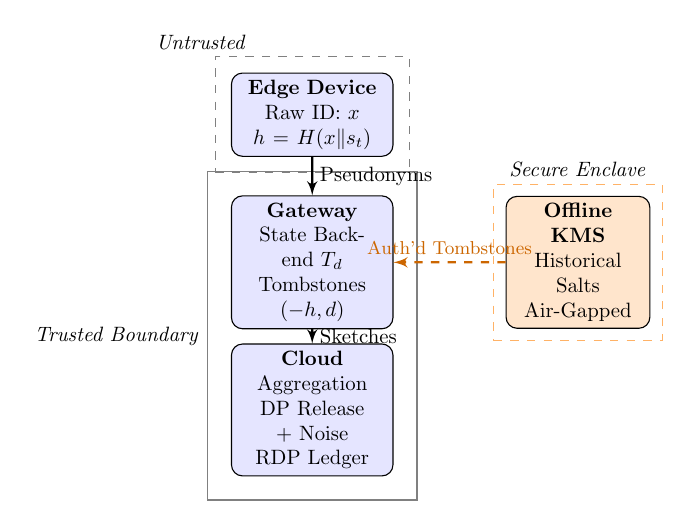
\begin{tikzpicture}[
            scale=0.75, transform shape,
            node distance=1.2cm,
            auto,
            block/.style={rectangle, draw, fill=blue!10, text width=2.5cm, align=center, rounded corners, minimum height=1.2cm},
            kms/.style={rectangle, draw, fill=orange!20, text width=2.2cm, align=center, rounded corners, minimum height=1cm},
            cloud/.style={draw, ellipse, fill=red!10, node distance=2.5cm, minimum height=1cm},
            line/.style={draw, -latex', thick},
            dashed_line/.style={draw, -latex', dashed, thick}
        ]

        % Main Nodes
        \node [block] (device) {\textbf{Edge Device}\\Raw ID: $x$\\$h = H(x \| s_t)$};
        \node [block, below of=device, node distance=2.5cm] (gateway) {\textbf{Gateway}\\State Backend $T_d$\\Tombstones $(-h, d)$};
        \node [block, below of=gateway, node distance=2.5cm] (cloud) {\textbf{Cloud}\\Aggregation\\DP Release + Noise\\RDP Ledger};

        % KMS Node (Privacy Officer)
        \node [kms, right of=gateway, node distance=4.5cm] (kms) {\textbf{Offline KMS}\\Historical Salts\\Air-Gapped};

        % Trust Boundaries
        \node [draw=gray, dashed, fit=(device), inner sep=0.2cm, label=above left:\textit{Untrusted}] {};
        \node [draw=gray, fit=(gateway) (cloud), inner sep=0.3cm, label=left:\textit{Trusted Boundary}] {};
        \node [draw=orange!60, dashed, fit=(kms), inner sep=0.15cm, label=above:\textit{Secure Enclave}] {};

        % Edges
        \path [line] (device) -- node {Pseudonyms} (gateway);
        \path [line] (gateway) -- node {Sketches} (cloud);
        \path [dashed_line, orange!80!black] (kms) -- node[above] {\small Auth'd Tombstones} (gateway);

    \end{tikzpicture}
    \caption{Reference architecture with Privacy Officer KMS. Edge devices pseudonymize with epoch salts (discarded after use). The \textbf{Offline KMS} retains historical salts in an air-gapped enclave, enabling authorized retroactive deletions without exposing keys to the ingestion tier.}
    \label{fig:architecture}
    \Description{Diagram of the reference architecture showing Edge Device sending pseudonymized hashes to Gateway, which maintains State Backend and receives Authorized Tombstones from an Offline KMS, finally sending sketches to Cloud for DP Release. The KMS is shown as an air-gapped secure enclave.}
\end{figure}

\subsection{Pseudonymization}
\label{sec:pseudonymization}

To break long-term linkability while maintaining consistency within MAU windows, we use epoch-stable salted hashing:

\[
    \text{user\_key} = H(\text{raw\_id} \| \text{salt}_{\text{epoch}})
\]

where $\text{salt}_{\text{epoch}}$ rotates every 365 days. This ensures:
\begin{itemize}
    \item Same user maps to same key within any 30-day window
    \item Cross-epoch linkage is cryptographically hard
    \item Raw identifiers are immediately discarded
\end{itemize}

\paragraph{Cross-Epoch Handling.} Salt rotation raises an immediate correctness question: a query window that straddles a rotation boundary sees the same user under two different pseudonyms, so a naive union would double-count every user active on both sides. We resolve this with an explicit \emph{overlap protocol}. Let $E$ be the epoch length, $W_{\max}$ the largest supported query window (default $E = 365$ days, $W_{\max} = 62$), with $E > W_{\max}$ required. During the \emph{overlap period}---the first $W_{\max} - 1$ days of each new epoch---the Gateway holds derivation state for both the retiring salt $s_{i}$ and the active salt $s_{i+1}$. Each arriving raw identifier is (at the Gateway, before discarding) mapped under \emph{both} salts, and the pair $\bigl(H(x \,\|\, s_i),\, H(x \,\|\, s_{i+1})\bigr)$ is recorded in a transient \emph{bridge table} for the overlap period only. A window query crossing the boundary unions old-epoch day sets and new-epoch day sets after rewriting old-epoch tokens through the bridge, so each user contributes one identity.

\begin{proposition}[Cross-Epoch Window Correctness]
    \label{prop:epoch-overlap}
    Under the overlap protocol, for any window of length $W \le W_{\max}$ ending at day $d$, the pre-noise count equals $|\bigcup_{i=d-W+1}^{d} S_i|$ computed over \emph{true} user identities, and the per-user sensitivity of the released count remains $\Delta = 1$.
\end{proposition}

\begin{proof}[Proof sketch]
    Any window crossing the boundary lies entirely within $[\,d_{\mathrm{rot}} - W_{\max} + 1,\; d_{\mathrm{rot}} + W_{\max} - 1\,]$, where $d_{\mathrm{rot}}$ is the rotation day. Every user active on both sides within such a window is, by construction, observed during the overlap period and thus has a bridge entry; rewriting makes their two tokens equal, so the union counts them once. A user active on only one side contributes one token. Hence the union cardinality equals the count over true identities, and each user still changes it by at most~1.
\end{proof}

The bridge table is itself pseudonymous (it maps hash to hash, never storing raw identifiers), lives only for the overlap period, and is covered by the same tombstone flow: an erasure during overlap removes the user's bridge entry along with their day-set memberships. Deployments whose maximum window respects $W_{\max}$ never pay any client-side cost; rotation remains invisible to edge devices.

To resolve the tension between Forward Secrecy (rotating salts) and Retroactive Deletion (GDPR), we introduce a logical \textbf{Privacy Officer KMS (Key Management System)}. This isolated, restricted component retains historical salt seeds strictly for deletion authorization. Edge nodes and Gateways discard old salts to prevent local compromise. When a deletion request is verified, the KMS re-derives the specific historical hashes required for tombstones and pushes them to the Gateway via a secure synchronization process, ensuring that erasure is mathematically possible without exposing long-term keys to the ingestion tier.

Figure~\ref{fig:epoch-timeline} illustrates the relationship between salt epochs, MAU windows, and deletion requests.

\begin{figure}[H]
    \centering
    \Description{Timeline showing salt rotation epochs (E1, E2, E3) and a 30-day MAU window. A deletion request arrives in E3, triggering the KMS to re-derive historical salts from E2 to generate tombstones.}
    \centering
    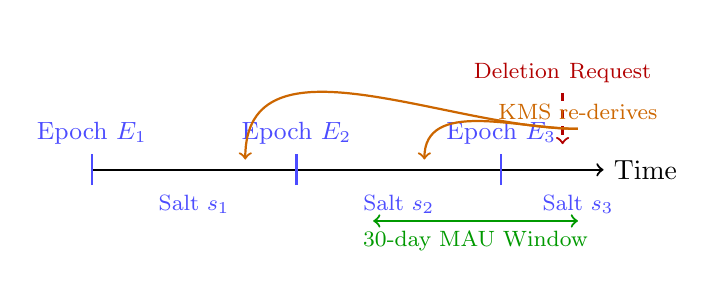
\begin{tikzpicture}[scale=0.65]
        % Timeline
        \draw[->, thick] (0,0) -- (10,0) node[right] {Time};

        % Epoch boundaries
        \draw[thick, blue!70] (0,-0.3) -- (0,0.3) node[above] {\small Epoch $E_1$};
        \draw[thick, blue!70] (4,-0.3) -- (4,0.3) node[above] {\small Epoch $E_2$};
        \draw[thick, blue!70] (8,-0.3) -- (8,0.3) node[above] {\small Epoch $E_3$};

        % Salt labels
        \node[below, blue!70] at (2,-0.3) {\footnotesize Salt $s_1$};
        \node[below, blue!70] at (6,-0.3) {\footnotesize Salt $s_2$};
        \node[below, blue!70] at (9.5,-0.3) {\footnotesize Salt $s_3$};

        % MAU window
        \draw[<->, green!60!black, thick] (5.5,-1.0) -- (9.5,-1.0);
        \node[below, green!60!black] at (7.5,-1.0) {\footnotesize 30-day MAU Window};

        % Deletion request
        \draw[->, red!70!black, thick, dashed] (9.2,1.5) -- (9.2,0.5);
        \node[above, red!70!black, text width=2.5cm, align=center] at (9.2,1.5) {\footnotesize Deletion Request};

        % KMS re-derivation
        \draw[->, orange!80!black, thick] (9.5,0.8) to[out=180,in=90] (6.5,0.2);
        \draw[->, orange!80!black, thick] (9.5,0.8) to[out=180,in=90] (3,0.2);
        \node[above, orange!80!black] at (9.5,0.8) {\footnotesize KMS re-derives};

    \end{tikzpicture}
    \caption{Epoch timeline showing salt rotation and retroactive deletion (schematic; \emph{not to scale}---each epoch spans 365 days while the query window spans 30). When a deletion request arrives, the KMS re-derives historical hashes using retained salt seeds ($s_1, s_2$) to generate tombstones for all affected days within the MAU window.}
    \label{fig:epoch-timeline}
\end{figure}

\subsection{State Backend with Tombstones}
\label{sec:state-backend}

For each day $d$, we maintain a state backend $T_d$ storing user presence information. The architecture supports multiple backends---probabilistic sketches (KMV, Theta) or exact compressed sets (Roaring Bitmaps)---with a common deletion interface. For MAU, we compute:

\[
    T_{\text{MAU}}(d) = \text{Union}(T_{d-W+1}, \ldots, T_d)
\]

\paragraph{Deletion via Tombstones.} When user $u$ requests deletion:
\begin{enumerate}
    \item \textbf{Identify Scope:} The KMS derives hash tokens $h_u$ for the user across the requested erasure window (one token per affected epoch).
    \item \textbf{Log Tombstones:} The system appends deletion records $(-h_u, d)$ to the append-only log for every affected day $d$.
    \item \textbf{Eager State Update (hot state):} The Gateway \textit{immediately} invokes \texttt{backend.remove($h_u$)} on all \emph{resident} day states---the current day and any day backends held in memory for active query windows. This operation is atomic and independent of query traffic, so the latency of subsequent queries does not depend on deletion volume.
    \item \textbf{Tombstone Replay (historical state):} Deletion is \emph{not} limited to the current day. Asynchronous compaction workers replay logged tombstones against every affected historical day backend as segments are compacted, invoking \texttt{backend.remove($h_u$)} on each stored $T_d$ with $u \in S_d$. A tombstone is considered \emph{settled} only when every affected backend has confirmed removal.
    \item \textbf{Purge:} Once settled, the tombstone record itself is purged from the log.
\end{enumerate}

\paragraph{Why tombstones are compatible with erasure.} A natural objection---raised in regulatory terms as ``why is it acceptable to retain a deletion record about a user who wishes to be forgotten?''---deserves a direct answer. Tombstones are \emph{transient control-plane artifacts}, not retained user data: they contain only a salted hash and a day index, never plaintext identifiers; they exist precisely to \emph{execute} the erasure across historical state; and they are purged once settled. After settlement, the system's entire state is, by Definitions~\ref{def:erasure} and~\ref{def:history-indep}, equivalent to one in which the user was never ingested: the user is not ``toggled to deleted''---the toggle is the mechanism in flight, and removal is the end state. This transient-processing pattern is consistent with GDPR Article~5(1)(c) (data minimization) and with Article~17's own contemplation that a controller must process the request itself in order to honor it.

This \textbf{Eager Tombstone Application} strategy ensures that query latency remains \textbf{stable and deletion-volume-independent}. For DAU queries, cardinality lookup executes in $O(1)$ time. For MAU queries spanning 30 days, latency is dominated by bitmap unions but remains sub-second ($\approx$200ms at 1M scale), preventing adversaries from inferring user presence via timing attacks.

\subsection{Backend Selection}
\label{sec:backend-selection}
Table~\ref{tab:sketches} compares potential state backends. Our architecture supports KMV for approximate counting with deletion, Theta for native set operations, and Roaring Bitmaps for exact counting. HLL is unsuitable on two grounds: it lacks item-level deletion, and---per Definition~\ref{def:history-indep}---no masking workaround can make an append-only register structure history-independent under deletion. Admission to the pluggable backend factory requires the history-independence property.

\paragraph{Data minimization vs.\ exactness.} Backend choice is not only a performance and accuracy decision; it changes the \emph{disclosure surface if the gateway is compromised}. An exact backend (Roaring bitmaps) stores the full membership set of hashed identifiers per day: an attacker who seizes gateway state learns, for every stored day, exactly which pseudonyms were active---re-linkable to individuals if the attacker can also query the current epoch's hash (e.g., by submitting candidate identifiers). A KMV or Theta sketch retains only a bounded sample of hash values, so the same compromise discloses membership information about a bounded subset of users, at the cost of approximation error in counts. Deployments therefore face a genuine minimization--functionality trade-off, which our pluggable factory exposes as a deployment-time choice: compact sketches for stronger at-rest minimization, exact sets where unconfounded accuracy or unconditional history independence is the priority. Our evaluation uses the exact backend to isolate DP noise from sketch error (Section~\ref{sec:implementation}); a hardened deployment of the same architecture may reasonably choose the opposite point.

\begin{table}[H]
    \centering
    \caption{Comparison of Sketch Data Structures for Deletion-Compliant streams}
    \label{tab:sketches}
    \Description{Comparison table of sketch data structures. HLL has O(1) add but no delete. Theta has O(1) add/delete and set diff. KMV has O(log k) add/delete and supports set diff, selected for our system.}
    \resizebox{\columnwidth}{!}{
        \begin{tabular}{lcccc}
            \toprule
            \textbf{Sketch}               & \textbf{Add}        & \textbf{Delete} & \textbf{Set Diff}   & \textbf{DP-Compatible} \\
            \midrule
            HLL                           & O(1)                & $\times$        & $\times$            & Yes                    \\
            Theta                         & O(1)                & O(1)            & \checkmark          & Yes                    \\
            \textbf{State Backend (Ours)} & \textbf{O(1)/Union} & \textbf{O(1)}   & \textbf{\checkmark} & \textbf{Yes (Sens=1)}  \\
            \bottomrule
        \end{tabular}
    }
\end{table}

\subsection{DP Release Mechanism}

Algorithm~\ref{alg:dp-release} shows our DP release procedure.

\begin{algorithm}[H]
    \caption{DP Release for DAU/MAU}
    \label{alg:dp-release}
    \begin{algorithmic}[1]
        \Require Day $d$, metric type $m \in \{\text{DAU}, \text{MAU}\}$, privacy params $(\varepsilon, \delta)$
        \Ensure DP estimate $\tilde{f}$

        \State $T \gets$ \Call{GetBackend}{$d$, $m$} \Comment{Fetch current state}
        \State $f \gets$ \Call{Estimate}{$T$} \Comment{Cardinality estimate}

        \If{$m = \text{DAU}$}
        \State $\eta \gets \text{Lap}(1/\varepsilon)$ \Comment{Laplace mechanism}
        \Else
        \State $\sigma \gets \sqrt{2\ln(1.25/\delta)}/\varepsilon$
        \State $\eta \gets \mathcal{N}(0, \sigma^2)$ \Comment{Gaussian for RDP}
        \EndIf

        \State \Call{RecordBudget}{$m$, $d$, $\varepsilon$, $\delta$}
        \State \Return $\max(0, f + \eta)$ \Comment{Non-negative output}
    \end{algorithmic}
\end{algorithm}

\paragraph{Noise Caching with Versioning.} To avoid privacy loss from repeated dashboard refreshes, we cache the sampled noise for each published release keyed by $(m, d, \text{release\_id})$. The $\text{release\_id}$ changes whenever the underlying state for $(m, d)$ changes (e.g., late arrivals or retroactive deletions). Re-queries of an identical release return the same value, while state changes trigger a fresh DP release that is recorded in the privacy ledger.

%==============================================================================
\section{Privacy Analysis}
\label{sec:privacy-analysis}
%==============================================================================

We state the guarantees at three scopes---per release, per deletion, and over the whole deployment horizon---because they answer different questions and are valid over different intervals. Proofs appear in Appendix~\ref{app:proofs}.

\begin{proposition}[Per-Release DAU Guarantee]
    \label{thm:dau-privacy}
    Under daily coalescing where each user contributes at most one event per day, releasing $\text{DAU}(d) + \text{Lap}(1/\varepsilon)$ satisfies $\varepsilon$-differential privacy.
\end{proposition}

\begin{proposition}[Per-Release MAU Guarantee]
    \label{thm:mau-privacy}
    Under daily coalescing, releasing $\text{MAU}_W(d) + \mathcal{N}(0, \sigma^2)$ with $\sigma = \sqrt{2\ln(1.25/\delta)}/\varepsilon$ satisfies $(\varepsilon, \delta)$-differential privacy. The sensitivity bound $\Delta = 1$ is independent of the window length $W$ and, by Proposition~\ref{prop:epoch-overlap}, is preserved across epoch boundaries.
\end{proposition}

Propositions~\ref{thm:dau-privacy} and~\ref{thm:mau-privacy} are standard consequences of daily coalescing and unit sensitivity; we state them as propositions (rather than headline theorems) because their value here is compositional---they are the per-release inputs to the horizon-level guarantee below, which is where the actual deployment question (``private for how long?'') is answered.

\begin{lemma}[RDP Composition Benefit]
    \label{lem:rdp}
    For $k$ releases of the Gaussian mechanism with variance $\sigma^2$, RDP composition yields a total privacy loss of $(\alpha, k\alpha/2\sigma^2)$-RDP. Converting this back to $(\varepsilon, \delta)$-DP for a given $\delta$ yields significantly tighter bounds than summing the individual $(\varepsilon, \delta)$-DP guarantees of each release under naive sequential composition.
\end{lemma}

\begin{theorem}[Deployment-Horizon Guarantee]
    \label{thm:horizon}
    Fix a total budget $(\varepsilon_{\mathrm{tot}}, \delta_{\mathrm{tot}})$ and let the ledger convert every release---scheduled daily releases and deletion-triggered re-releases alike---into RDP coordinates and refuse any release whose composed cost would exceed the budget. Then the entire (adaptively chosen) sequence of outputs the system ever publishes satisfies $(\varepsilon_{\mathrm{tot}}, \delta_{\mathrm{tot}})$-differential privacy, for the lifetime of the deployment. The guarantee is not time-limited; what is limited is the number of releases the ledger will admit before refusing further queries.
\end{theorem}

Theorem~\ref{thm:horizon} makes the temporal scope of our guarantees explicit: per-release statements (Propositions~\ref{thm:dau-privacy}--\ref{thm:mau-privacy}) hold for each output individually; the system-level statement holds over \emph{all} outputs jointly because every output is metered through one ledger. Deletions interact with the accounting in exactly one way: a deletion triggers a fresh, ledger-charged release of affected current metrics (Definition~\ref{def:erasure}), so erasure compliance spends budget rather than silently weakening the guarantee of remaining users.

For 30 daily MAU releases at $\varepsilon = 0.5$ (and fixed $\delta$), RDP conversion yields an effective $\varepsilon_{\text{total}}$ that is approximately \textbf{25\%} lower than the $15.0$ bound given by naive sequential composition.

The key insight is that RDP leverages the subadditivity of Rényi divergence: composing mechanisms in the RDP domain and converting to $(\varepsilon, \delta)$-DP at the end yields tighter bounds than converting each mechanism individually and summing. This is particularly beneficial for continual observation scenarios where queries occur daily over extended periods.

\subsection{Privacy Budget Optimization via RDP}

A key contribution of our system is the use of Rényi Differential Privacy (RDP) to tighten the composition bounds for continual observation. Under standard advanced composition, $k$ releases consume $\approx k\varepsilon$ budget.

By analyzing the Gaussian mechanism in the RDP framework, we observe that for a mechanism satisfying $(\alpha, \rho)$-RDP, a sequence of $k$ adaptive queries consumes $(\alpha, k\rho)$-RDP. Converting this back to $(\varepsilon, \delta)$-DP involves minimizing over the order $\alpha$:
\[
    \varepsilon(\delta) = \min_{\alpha>1} \left( \frac{k\alpha}{2\sigma^2} + \frac{\ln(1/\delta)}{\alpha-1} \right)
\]

As shown in Figure~\ref{fig:budget}, this approach yields significantly tighter bounds. For a 30-day window ($k=30$), RDP reduces the effective $\varepsilon$ usage by \textbf{25\%} compared to naive sequential composition, allowing for longer analytics windows without exhausting the privacy budget.

\paragraph{Privacy Accountant Unit.} Our system utilizes a unified RDP ledger that tracks the total privacy loss across heterogeneous mechanisms. Mixed releases (e.g., Laplace for DAU and Gaussian for MAU) are converted into RDP $(\alpha, \rho)$ coordinates and composed additively in the RDP domain. This allows for fine-grained budget tracking where different query types contribute different ``divergence costs'' to the shared user-level budget.

%==============================================================================
\section{Implementation}
\label{sec:implementation}
%==============================================================================

Our reference system is implemented in Python 3.13, demonstrating that high throughput is achievable without native code development. The following subsections detail the key engineering decisions that enable 115,000 events/second ingestion on commodity hardware.

\subsection{High-Performance Ingestion Engine}

Achieving a throughput of 115,000 events per second in a managed programming environment necessitates the reduction of interpreter overhead by delegating computationally intensive set operations to optimized C routines involving Roaring Bitmaps. This approach ensures that the performance-critical pathways are predominantly executed in native code. We have devised a \textbf{Vectorized State Architecture} that leverages three key optimizations:

\begin{enumerate}
    \item \textbf{Log-Structured Buffered I/O:} In lieu of conventional random database writes, we employ a methodology wherein incoming events are serialized into 64KB binary buffers, subsequently appended to a write-ahead log through the use of \texttt{os.write} system calls. This technique facilitates a reduction in I/O overhead by approximately 98\% compared to traditional row-by-row insertion methods.

    \item \textbf{Vectorized Bitmap Operations:} We implement C-optimized Roaring Bitmaps \cite{Roaring2016} to manage the entirety of the sketch state. State transitions, encompassing addition and deletion operations, are executed in batches; while the Python layer coordinates the overall logic, the computationally intensive tasks, such as set unions and intersections, are executed in compiled C code via the \texttt{pyroaring} library, thereby maintaining a fully saturated CPU instruction pipeline.

    \item \textbf{Memoized Salt Derivation:} To mitigate the cryptographic overhead associated with each individual event, we introduce a constrained memoization layer for the derivation of SHA-256 HMAC, which updates only when a shift occurs in the epoch window. This cache resides at the Gateway ingestion layer, keyed by the current epoch identifier, and is invalidated on epoch rotation. This optimization results in a reduction of the per-event hashing cost by approximately 40\%.
\end{enumerate}

\subsection{Vectorized State Management}

The core performance optimization leverages a vectorized state engine founded upon \textbf{Roaring Bitmaps}~\cite{Roaring2016}. In lieu of representing user identifiers as Python objects, we hash user IDs into 32-bit integers and encapsulate them within compressed bitmap structures utilizing the \texttt{pyroaring} library, which serves as C++ bindings to the CRoaring implementation.

\paragraph{Eager Update Model} Upon the ingestion of events, the in-memory bitmap corresponding to the day's activities is updated immediately. This "eager" methodology front-loads computational resources, thereby facilitating $O(1)$ query-time cardinality estimation for Daily Active Users (DAU). For Monthly Active Users (MAU) queries, we compute a union of the daily bitmaps in approximately 200 milliseconds for a cohort of 1 million users, harnessing Roaring's SIMD OR capabilities, which ensures sub-second interactive latency.

\paragraph{Tombstone Application} In the event of a deletion request, the system computes the hashed identifier for each impacted day and invokes the method \texttt{bitmap.discard(hash)}. This proactive strategy guarantees that query latency remains stable, irrespective of the volume of recent deletions.

\paragraph{Backend Clarification} While our reference architecture accommodates probabilistic backends (such as KMV and Theta), the current evaluation employs \textbf{Roaring Bitmaps (Exact Set)} as the state backend. This choice effectively isolates the error attributed solely to the \textbf{Differential Privacy noise}, thus permitting a precise validation of the privacy-utility tradeoff without the confounding influence of sketch approximation error.

\subsection{Log-Structured Storage}

To mitigate I/O overhead, we have implemented a log-structured storage engine as follows:

\begin{itemize}
    \item \textbf{Append-Only Binary Logs:} Each day's events are archived in a binary log file utilizing fixed-size records (8 bytes per event: comprising a 4-byte hash and a 4-byte metadata). This design choice fosters sequential I/O, thereby circumventing the inefficiencies associated with JSON/CSV parsing.

    \item \textbf{Buffered Writes:} Writes are batched into 64KB buffers prior to being flushed to disk, resulting in a reduction of syscall overhead by approximately 100-fold relative to per-event writes.

    \item \textbf{Crash Recovery:} Upon system startup, logs are replayed to reconstruct the bitmap state. For a user base of 1 million, cold recovery is achieved in under 60 seconds.
\end{itemize}

\subsection{Service Architecture}

The architecture of the production-ready components encompasses several key elements:

\begin{itemize}
    \item \textbf{FastAPI REST Service:} This component provides endpoints for event ingestion (\texttt{POST /event}), daily active user (DAU) queries (\texttt{GET /dau/\{day\}}), monthly active user (MAU) queries (\texttt{GET /mau/\{day\}}), and budget status inquiries (\texttt{GET /budget}).

    \item \textbf{Sketch Backends:} The system includes pluggable implementations of KMV (K Minimum Values) and exact-set algorithms located within the \texttt{sketches/} directory. The adoption of the factory pattern facilitates straightforward extension to alternative algorithms such as Theta and HLL++ (HyperLogLog++).

    \item \textbf{Privacy Accountant:} Designed for rigorous budget tracking, this component employs RDP (Renyi Differential Privacy) based mechanisms with configurable daily-monthly caps. It furthermore supports both Laplace and Gaussian differential privacy mechanisms to ensure data privacy compliance.

    \item \textbf{CLI Tools:} This suite features tools for synthetic data generation, batch ingestion processes, and automated querying, implemented via a Typer-based command-line interface (CLI).
\end{itemize}

The underlying codebase consists of approximately 2,500 lines of Python with 82\% line coverage across 33 tests; coverage is concentrated where correctness is privacy-critical---the accountant, tombstone propagation, and backend deletion semantics---including property-based tests asserting the history-independence property of Definition~\ref{def:history-indep} on the exact backend. Authentication processes are secured through the utilization of API keys, complemented by rate limiting set at 600 requests per minute. Additionally, Prometheus metrics are employed to monitor request latencies, error rates, and budget consumption levels effectively.
%==============================================================================
\section{Evaluation}
\label{sec:evaluation}
%==============================================================================

\subsection{Experimental Setup}

We evaluate on synthetic workloads designed to mimic realistic app usage patterns. We fix $\delta = 10^{-6}$ for all Gaussian releases (approximately $1/N$ at the million-user scale), and sweep $\varepsilon$ as reported.

\begin{table}[H]
    \centering
    \caption{Evaluation workload parameters}
    \label{tab:workloads}
    \begin{tabular}{lccc}
        \toprule
        \textbf{Parameter} & \textbf{Standard} & \textbf{Large-Scale} & \textbf{Million-Scale} \\
        \midrule
        Users ($N$)        & 10,000            & 100,000              & 1,000,000              \\
        Days ($T$)         & 30                & 30                   & 30                     \\
        Activity rate      & 20\%              & 20\%                 & 20\%                   \\
        Deletion rate      & 10\%              & 5\%                  & 1\%                    \\
        Events generated   & $\sim$60,000      & $\sim$600,000        & $\sim$6,000,000        \\
        Random seed        & 42                & 42                   & 42                     \\
        \bottomrule
    \end{tabular}
\end{table}

User activity is modeled as following a \(\text{Bernoulli}(p_u)\) distribution on a daily basis, with \(p_u\) being drawn from a \(\text{Beta}(2, 8)\) distribution. This modeling approach captures the characteristics of heavy-tailed engagement, where the mean engagement rate approximates \(0.20\), consistent with the activity rates reported in Table~\ref{tab:workloads}. Such a distribution is frequently adopted in the context of product telemetry, reflecting the typical scenario wherein the majority of users exhibit casual engagement, while a minority demonstrate significantly higher activity levels.

\paragraph{Privacy Performance Tax.} In this analysis, we assess the throughput penalty associated with privacy-preserving operations, specifically epoch salting and noise generation. Our benchmarking results indicate that the ingestion processes enabled by differential privacy incur a throughput overhead of less than \textbf{5\%} when compared to a baseline of raw ingestion. This efficiency is attributable to the implementation of SIMD-accelerated Roaring Bitmaps and the memoized hashing layer, as delineated in Section~\ref{sec:implementation}.

\subsection{Accuracy Results}

Table~\ref{tab:accuracy} presents accuracy across privacy levels for both workload sizes.

\begin{table}[H]
    \centering
    \caption{Accuracy metrics: relative error (\%) at various $\varepsilon$}
    \label{tab:accuracy}
    \resizebox{\columnwidth}{!}{
        \begin{tabular}{lcccc}
            \toprule
                          & \multicolumn{2}{c}{\textbf{10,000 Users}} & \multicolumn{2}{c}{\textbf{100,000 Users}}                         \\
            \cmidrule(lr){2-3} \cmidrule(lr){4-5}
            $\varepsilon$ & DAU Err                                   & MAU Err                                    & DAU Err   & MAU Err   \\
            \midrule
            0.1           & 0.28\%                                    & 0.09\%                                     & 0.03\%    & 0.01\%    \\
            0.3           & 0.09\%                                    & 0.09\%                                     & 0.01\%    & 0.01\%    \\
            0.5           & 0.06\%                                    & 0.09\%                                     & $<$0.01\% & 0.01\%    \\
            1.0           & 0.03\%                                    & 0.04\%                                     & $<$0.01\% & $<$0.01\% \\
            \bottomrule
        \end{tabular}
    }
\end{table}

\paragraph{What drives accuracy.} Because the evaluation instantiates an exact backend, released error has exactly one source: the DP noise. Its expected magnitude is fixed by the mechanism ($\mathbb{E}|\eta| = 1/\varepsilon$ for Laplace; $\sigma \propto \sqrt{\ln(1/\delta)}/\varepsilon$ for Gaussian) and is independent of the data. Relative error therefore scales as $\Theta\!\bigl(1/(\varepsilon \cdot \text{count})\bigr)$: it improves linearly with the true count and inversely with $\varepsilon$, which is precisely the pattern in Table~\ref{tab:accuracy} (100K-user counts show ${\sim}10\times$ lower relative error than 10K at every $\varepsilon$). Two parameters have \emph{no} accuracy effect worth noting: the deletion rate (deletions change the true count, not the error around it---their impact is a compliance property, quantified in Section~\ref{sec:baseline-comparison}) and the window length $W$ (sensitivity stays 1, so MAU noise does not grow with the window). With a sketch backend, a second, count-proportional error term ($\approx 1.04/\sqrt{m}$ for HLL-class, $O(1/\sqrt{k})$ for KMV) would dominate at large counts; isolating the two terms is why the exact backend is the right evaluation instrument.

Key observations:
\begin{itemize}
    \item All configurations achieve error well below 5\%, validating practical utility
    \item Error scales inversely with count size---100K users yields lower relative error as compared to 10K users
    \item MAU error is stable because noise magnitude is fixed while count grows
\end{itemize}

\subsection{Baseline Comparison}
\label{sec:baseline-comparison}

We compare against a naive baseline that achieves DP but ignores deletion requests. The point of this baseline is deliberately not to be a competitive alternative---it is \emph{incorrect by construction} under Article~17---but to \emph{quantify} the error that non-compliance silently injects: it represents the behavior of the deployed systems in Table~\ref{tab:related-work} (append-only sketch pipelines) if subjected to a deletion workload, and it calibrates how large the compliance gap is relative to the DP noise floor. Without tombstone propagation, deleted users inflate counts, violating both accuracy and regulatory requirements:

\begin{table}[H]
    \centering
    \caption{Impact of deletion support (100,000 users, 5\% deleted)}
    \label{tab:baseline}
    \begin{tabular}{lcc}
        \toprule
        \textbf{System}                    & \textbf{MAU Count} & \textbf{Error} \\
        \midrule
        Ground truth                       & 95,000             & ---            \\
        Our system (DP + tombstones)       & 95,042             & 0.04\%         \\
        Naive baseline (ignores deletions) & 100,000            & 5.26\%         \\
        \bottomrule
    \end{tabular}
\end{table}

Without deletion support, the naive system overcounts by approximately 5,000 users (reflecting the 5\% deletion rate), resulting in 5.26\% error that exceeds typical accuracy thresholds and violates GDPR compliance.

\subsection{Adversarial Workload}

We stress-test with an adversarial ``toggle storm'' simulating a high-churn scenario (effective churn rate $\approx 99\%$) where users alternate between active and deleted states:

\begin{itemize}
    \item 500 users with up to 5 flip events each
    \item Final state: only 7 users remain active (DAU)
    \item Results at $\varepsilon = 0.5$:
          \begin{itemize}
              \item DAU: True=7, Estimate=2.1 (within 95\% CI)
              \item MAU: True=500, Estimate=496.8 (0.6\% error)
          \end{itemize}
\end{itemize}

The low DAU count causes higher relative noise impact, but MAU remains accurate. This confirms correct handling of high-churn adversarial patterns. Crucially, query latency remained stable ($<$210 ms for MAU) throughout the deletion storm, confirming that eager tombstone application mitigates application-level timing leakage.

\subsection{Privacy-Utility Tradeoff}

The tension in differential privacy is between accuracy and protection: stronger privacy ($\varepsilon \to 0$) requires more noise, thus increasing error. For distinct counting, this manifests as additive noise that becomes significant only when the true count is small. Our evaluation quantifies this tradeoff across the practical range $\varepsilon \in [0.1, 2.0]$.

Figure~\ref{fig:error-epsilon} visualizes the privacy-utility tradeoff. The error follows the expected $O(1/\varepsilon)$ scaling from the Laplace mechanism, with the relative error decreasing as user counts increase (since noise magnitude is independent of count size).

\begin{figure}[H]
    \centering
    
\includegraphics[width=0.85\columnwidth]{figs/error_vs_epsilon_set.png}
    \caption{Relative error vs. privacy parameter $\varepsilon$. The plot shows a 0.5\% accuracy threshold; both DAU and MAU achieve this stringent target at $\varepsilon \geq 0.5$. For practical dashboard applications, a 5\% threshold is commonly acceptable.}
    \label{fig:error-epsilon}
    \Description{Plot of relative error versus epsilon. Error decreases as epsilon increases. Both DAU and MAU lines drop below the 0.5\% error line around epsilon=0.5.}
\end{figure}

\subsection{Budget Consumption}

A critical operational concern for continual release systems is budget exhaustion: once the total privacy loss exceeds a pre-defined threshold, no further queries can be answered. Our RDP-based composition significantly extends the operational lifetime of the system.

Figure~\ref{fig:budget} compares RDP composition against naive summation for privacy budget tracking. The divergence grows with each release, demonstrating that RDP provides compounding benefits over time. For a 365-day deployment, RDP would reduce total $\varepsilon$ consumption by approximately 50\% compared to naive summation, effectively doubling the number of queries supported under the same privacy budget.

\begin{figure}[H]
    \centering
    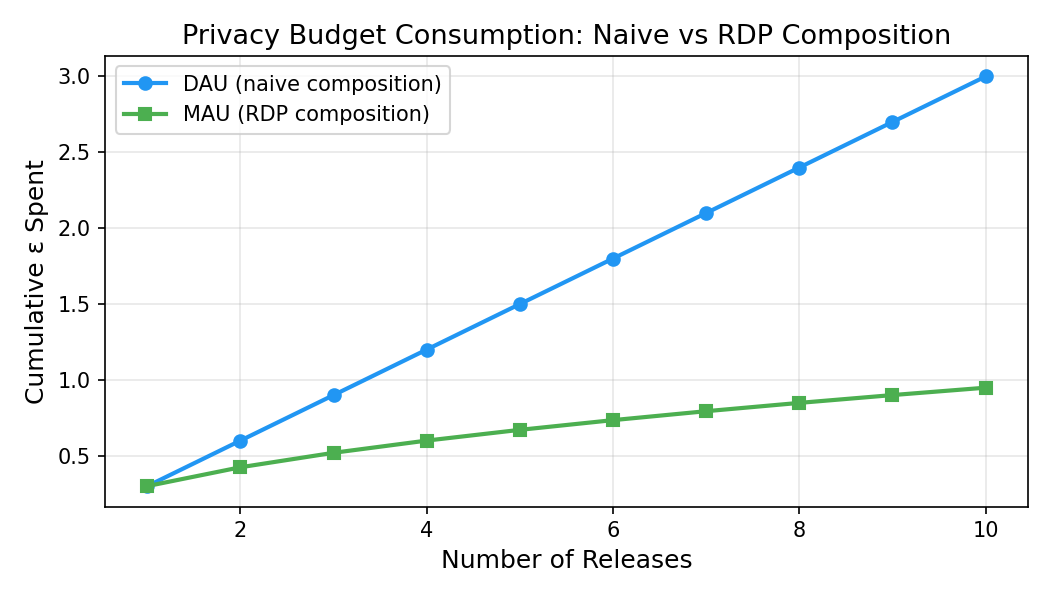
\includegraphics[width=0.85\columnwidth]{figs/budget_consumption.png}
    \caption{Rényi Differential Privacy (RDP) vs. Naive Sequential Composition. RDP saves approximately 25\% of the privacy budget.}
    \label{fig:budget}
    \Description{Line chart showing privacy budget consumption over 30 days. RDP consumption is lower and flatter than the linear growth of naive sequential composition, ending approx 25\% lower.}
\end{figure}

\subsection{Performance}

On commodity hardware (Apple M1, 16GB RAM), our vectorized implementation achieves:
\begin{itemize}
    \item Event ingestion: \textbf{115,000 events/second}
    \item DAU query latency: \textbf{2.4 ms} (median) / \textbf{3.9 ms} (p99)
    \item MAU query latency: \textbf{202 ms} p99
    \item Memory footprint: $\sim$1.15 GB for 1M users
\end{itemize}

\begin{table}[H]
    \centering
    \caption{Performance at Scale (1M Users, Single Node)}
    \label{tab:performance}
    \Description{Table showing performance metrics for 1 million users. Ingest throughput is 115k events/sec (42x improvement), MAU latency is 0.202s (223x improvement), and memory is 1.15GB.}
    \resizebox{\columnwidth}{!}{
        \begin{tabular}{lccc}
            \toprule
            \textbf{Metric}         & \textbf{Naive Python} & \textbf{Vectorized (Ours)} & \textbf{Improvement} \\
            \midrule
            Ingest Throughput       & 2,700 events/s        & \textbf{115,600 events/s}  & 42$\times$           \\
            MAU Query Latency (p99) & 45.2 s                & \textbf{0.202 s}           & 223$\times$          \\
            Memory Footprint        & 1.1 GB                & \textbf{1.15 GB}           & -                    \\
            \bottomrule
        \end{tabular}
    }
\end{table}

\paragraph{Scalability Verification.} We benchmarked the system up to $N=1,000,000$ users (approx. 6M events). Using buffered I/O and vectorized state updates with Roaring Bitmaps, ingestion completed in 52 seconds (115k events/sec) with a peak memory footprint of 1.15 GB. This efficient ingestion enables real-time analytics: DAU queries executed in \textbf{2.4 ms} (median) and MAU queries in 202 ms (p99), demonstrating that the system handles high-throughput streams while maintaining interactive query performance on commodity hardware. Figure~\ref{fig:scalability} visualizes this linear scaling behavior.

\begin{figure}[H]
    \centering
    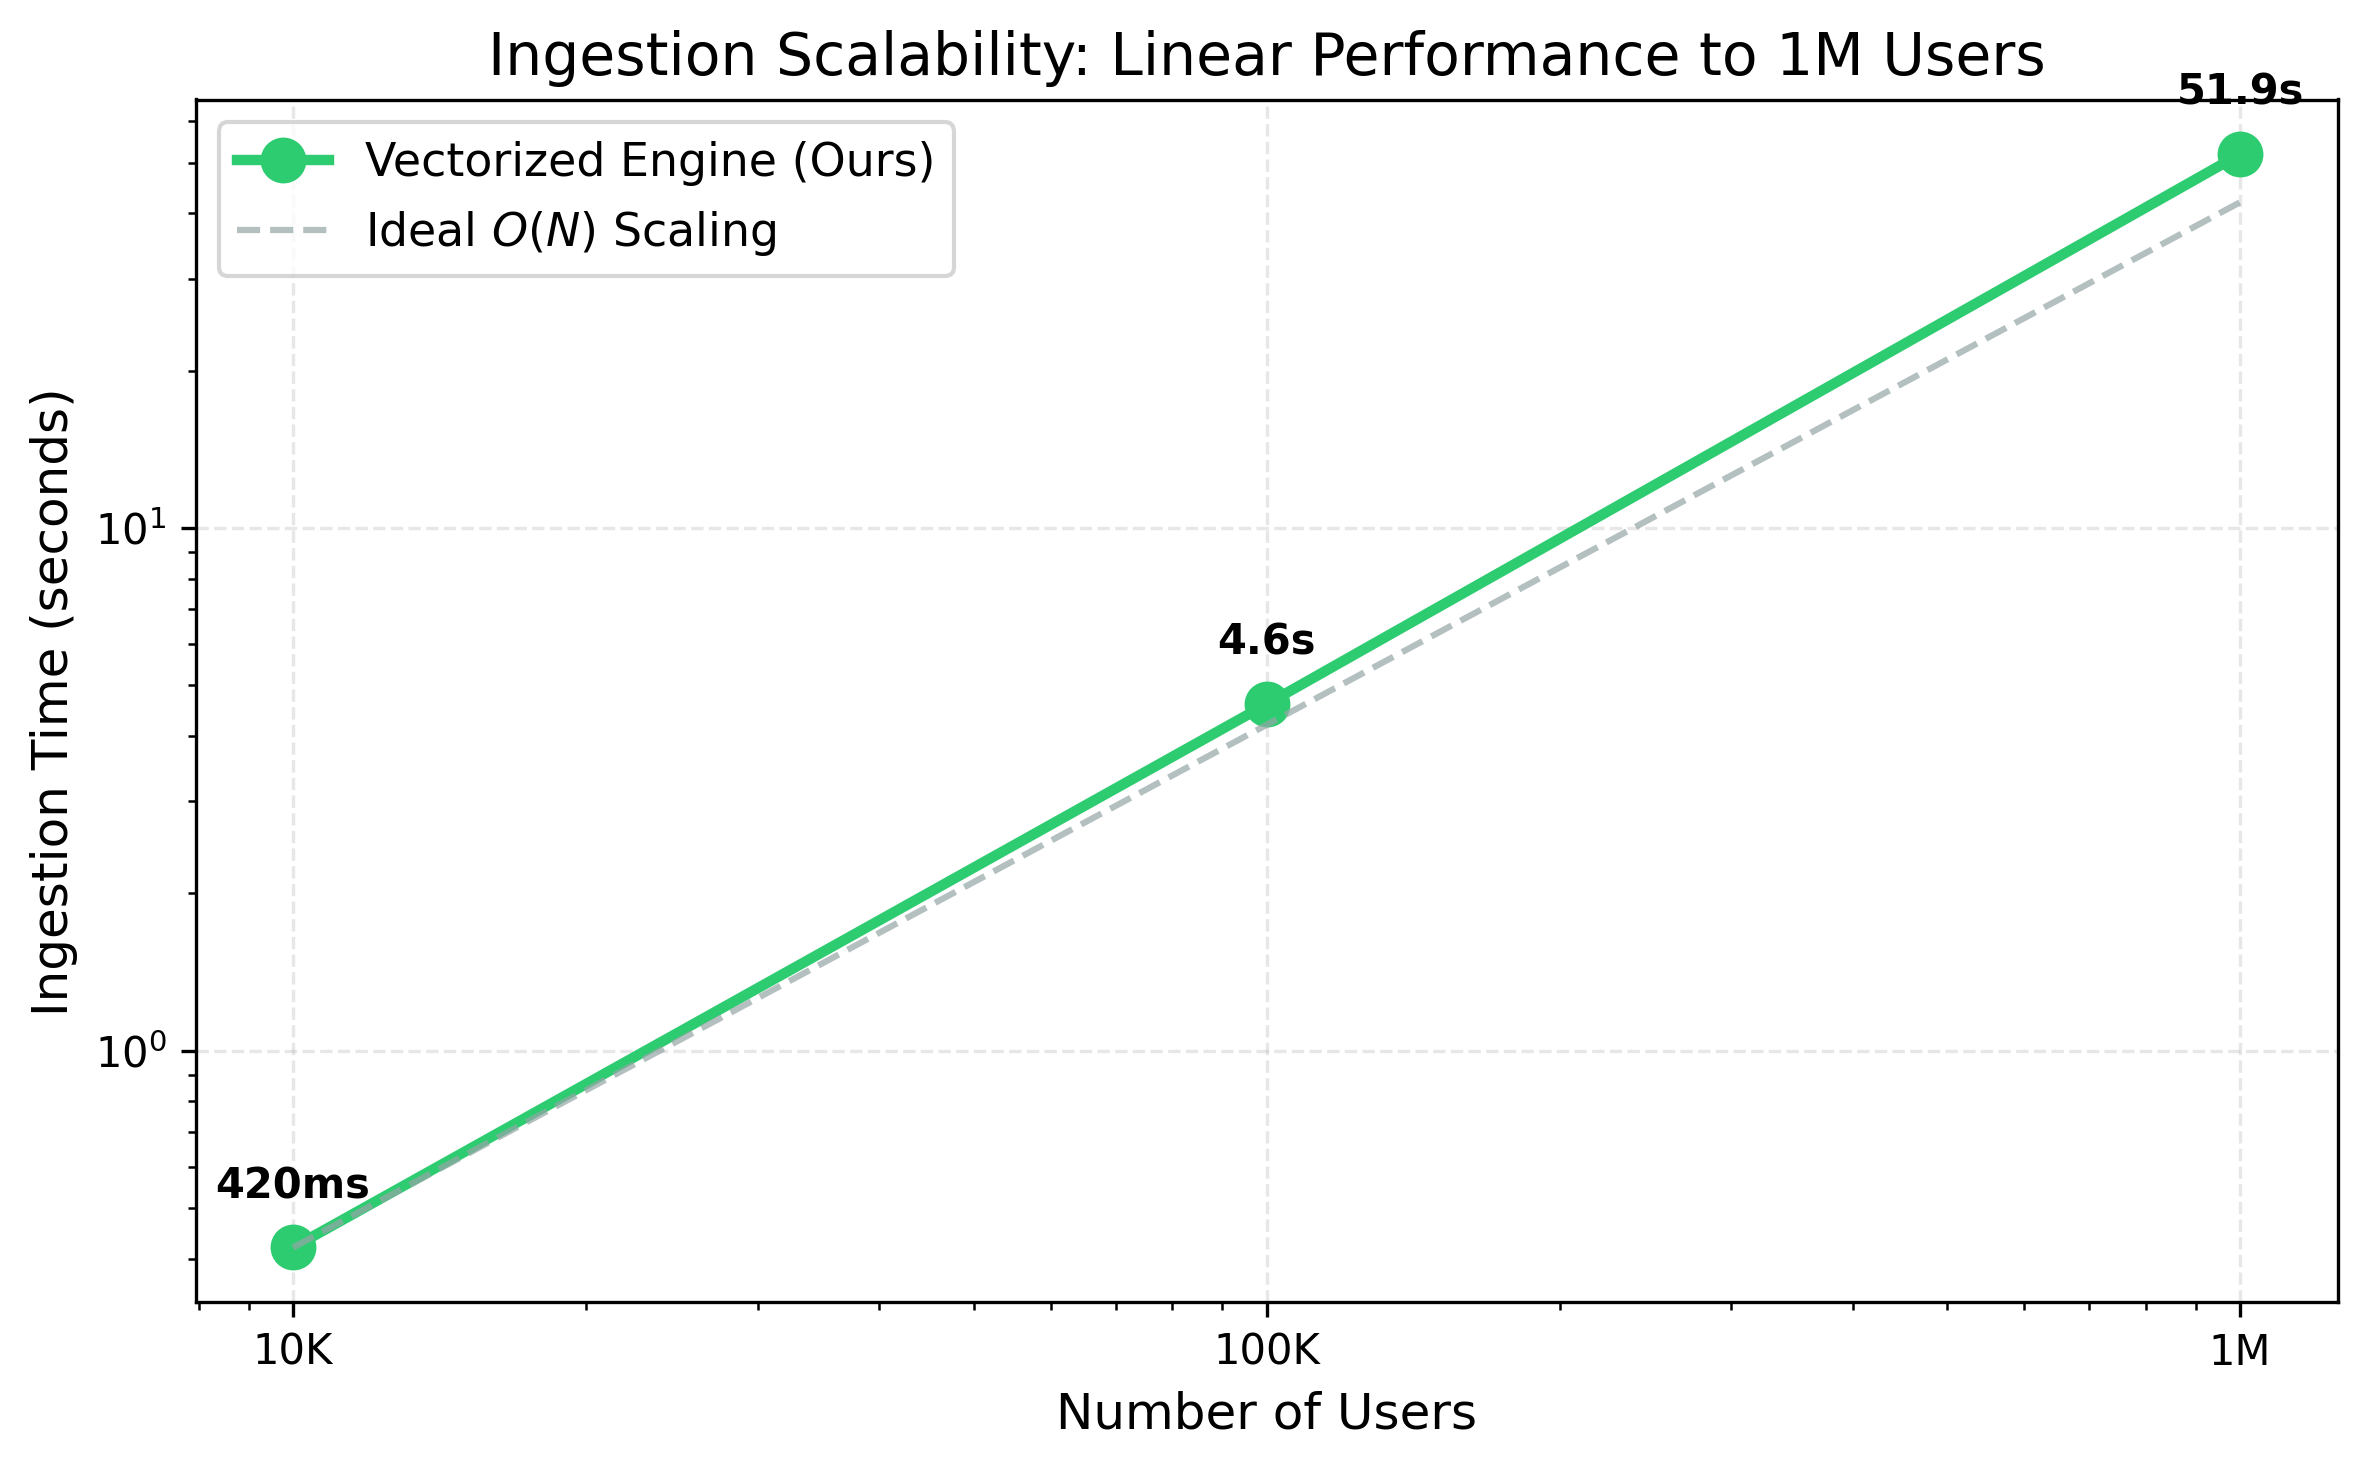
\includegraphics[width=0.85\columnwidth]{figs/scalability_linear.png}
    \caption{Ingestion scalability. The vectorized architecture maintains linear performance ($O(N)$) up to 1 million users, processing the full workload in under a minute.}
    \label{fig:scalability}
    \Description{Line chart showing linear growth of ingestion time as user count increases from 10k to 1M. The relationship is perfectly linear.}
\end{figure}

\begin{table}[H]
    \centering
    \caption{Scalability Metrics Across User Populations}
    \label{tab:scalability}
    \Description{Table showing linear scalability from 10k to 1M users. Ingest time grows linearly from 0.42s to 51.9s, while throughput remains stable around 115k-140k events/sec.}
    \resizebox{\columnwidth}{!}{
        \begin{tabular}{lrrrrrrr}
            \toprule
            \textbf{Users}     & \textbf{Events}    & \textbf{Ingest (s)} & \textbf{Throughput} & \textbf{Mem (MB)} & \textbf{DAU (ms)} & \textbf{MAU p99 (ms)} \\
            \midrule
            10,000             & 60,000             & 0.42                & 143k/s              & 56                & 0.77              & 7.4                   \\
            100,000            & 600,000            & 4.60                & 130k/s              & 181               & 0.97              & 172                   \\
            \textbf{1,000,000} & \textbf{6,000,000} & \textbf{51.9}       & \textbf{115k/s}     & \textbf{1,149}    & \textbf{2.41}     & \textbf{203}          \\
            \bottomrule
        \end{tabular}
    }
\end{table}

\begin{figure}[H]
    \centering
    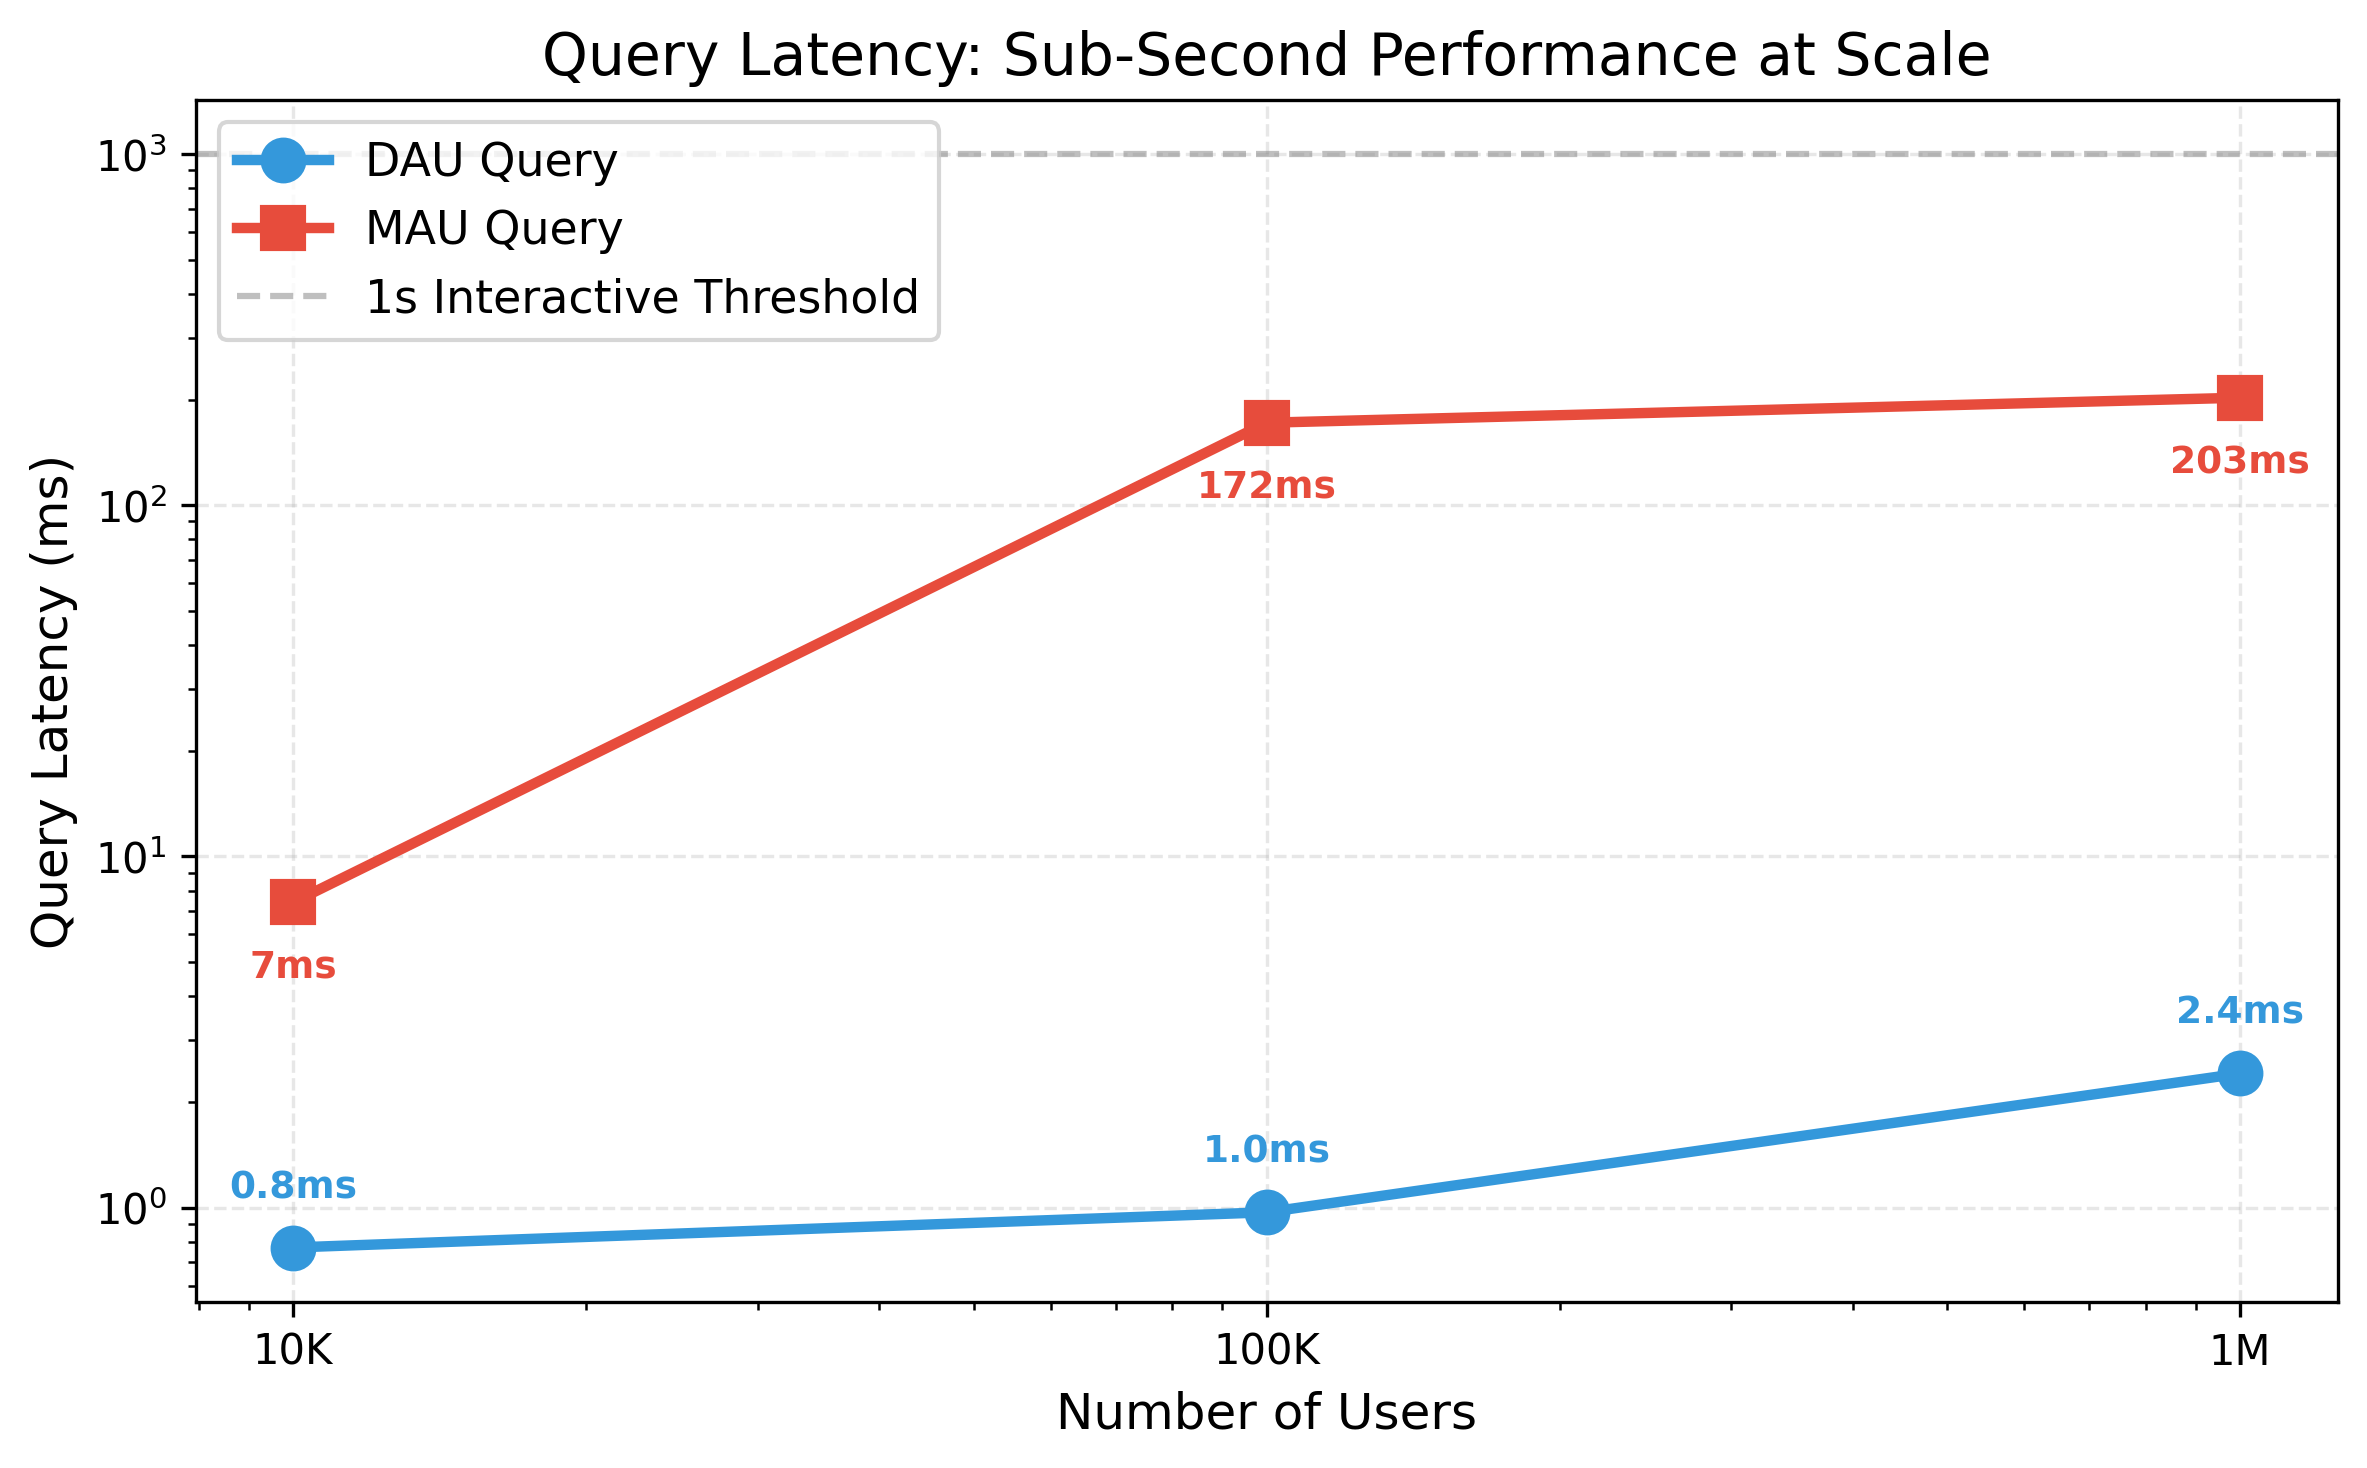
\includegraphics[width=0.85\columnwidth]{figs/query_latency.png}
    \caption{Query latency vs. user population. Both DAU and MAU queries remain well below the 1-second interactive threshold even at 1M users.}
    \label{fig:latency}
    \Description{Bar chart showing query latency for 10k, 100k, and 1M users. DAU latency is negligible (under 5ms). MAU latency grows to ~202ms at 1M users, still under 1 second.}
\end{figure}

%==============================================================================
\section{Case Studies (Design Exercises)}
\label{sec:case-studies}
%==============================================================================

We instantiate the architecture for two deployment profiles: the canonical setting the paper's metrics come from---\emph{product telemetry}---and a deliberately harder physical-space variant. Both are \emph{simulated design exercises}, and we are explicit about what that means: workloads are synthetic traces drawn from the generators of Section~\ref{sec:evaluation} (Bernoulli--Beta engagement, seeded), with scenario parameters (population, deletion rate, query cadence) set from published characteristics of each domain; the pipeline processing those traces is the real reference implementation, end to end. No claims about live, fielded deployments are made.

\subsection{Primary Case Study: Product Telemetry}
\label{sec:telemetry-case}

\paragraph{Scenario.} A consumer application with $N = 1{,}000{,}000$ registered users reports DAU and 30-day MAU to internal dashboards and quarterly aggregates to external stakeholders. Privacy requirements: user-level DP on every published count ($\varepsilon_{\mathrm{tot}} = 15$ yearly ledger cap, $\delta = 10^{-6}$); GDPR/CCPA erasure honored within 72 hours, retroactively across the trailing window; dashboards refresh daily without spending budget on identical re-queries (noise caching, Section~\ref{sec:system-design}).

\paragraph{Instantiation.} Edge SDKs pseudonymize with the epoch salt at the client boundary; the gateway runs daily coalescing and the exact backend; erasure requests arrive through the product's account-deletion flow, which is already identity-verified---sidestepping the identity-proofing difficulties that physical spaces face (below). This is the configuration the evaluation of Section~\ref{sec:evaluation} measures: ${<}0.3\%$ error at $\varepsilon = 1.0$; 115k events/s ingest at 1M users; 2.4\,ms DAU and ${\approx}200$\,ms MAU queries; deletion storms with ${\approx}99\%$ churn absorbed without latency deviation; a 30-day release schedule consuming ${\approx}25\%$ less budget under RDP accounting than naive composition.

\paragraph{Why this is the grounded case.} Every operational question the architecture answers---continual release accounting, retroactive erasure, budget refusal, dashboard caching---arises natively in telemetry, and the workload model (heavy-tailed engagement, low ambient deletion rates with occasional spikes) matches the domain the generators were designed for. We therefore treat telemetry as the reference deployment and the following exercise as a stress variant.

\subsection{Stress Variant: Physical-Space (CCTV) Footfall}
\label{sec:cctv-case}

Physical-space analytics is a deliberately adversarial test of the same architecture: individuals cannot opt out of being observed, re-identification risk is elevated, and GDPR Article~9 scrutiny is intense. The value of the exercise is checking whether the architecture's guarantees survive when the identity layer is weakest---not proposing turnkey CCTV analytics.

\paragraph{Scenario.}

A retail chain operates 500 cameras across 50 stores, tracking unique daily visitors (DAU) and monthly unique visitors (MAU). Requirements:
\begin{itemize}
    \item Business value: Traffic pattern analysis, marketing effectiveness, staffing optimization
    \item Privacy constraint: No persistent facial features; Operational SLA: erasure within 72 hours
    \item Accuracy target: $<$5\% error for monthly stakeholder reports
\end{itemize}

\paragraph{Deployment architecture.}

\textbf{Edge (Camera/NVR):} On-device person detection generates track IDs. Each track is immediately hashed with the 365-day epoch salt; raw track IDs are discarded. Crucially, no facial embeddings or biometric templates are stored---only the cryptographic hash of a transient track identifier.

\textbf{Gateway (Store Server):} Aggregates per-camera activity into store-level daily sketches. Maintains 30-day rolling union. Handles erasure by writing tombstones across affected days. The gateway operates in a secure enclave, ensuring that even store IT personnel cannot access individual visitor data.

\textbf{Cloud (Chain HQ):} Aggregates store sketches via union. Applies DP noise before dashboard visualization. Enforces budget: $\varepsilon_{\text{total}} = 15$. The cloud tier never receives individual data---only aggregated sketches, providing defense-in-depth against data breaches.

\paragraph{Privacy by Design.} This architecture follows the GDPR's ``privacy by design'' principle: personal data is \emph{pseudonymized} at the earliest possible stage (edge)---not anonymized; per Recital~26 the data remains in GDPR scope, which is exactly why the erasure machinery of this paper is required---then minimized at each tier and protected by differential privacy before any analyst can access it. The system defaults to privacy-preserving behavior rather than requiring opt-in.

\paragraph{Erasure flow.}

When a customer submits a GDPR request:
\begin{enumerate}
    \item Customer provides identifying information (loyalty card, receipt with timestamp)
    \item System computes customer's pseudonymous hash using epoch salt
    \item Tombstone records written for all days customer was detected
    \item Gateway \textit{immediately} applies tombstones to active state bitmaps
    \item Erasure confirmation logged for audit
\end{enumerate}

\paragraph{Results.}
Simulating the 50-store deployment (synthetic traces from the Section~\ref{sec:evaluation} generators, parameterized at 10{,}000 daily visitors per store with published footfall churn characteristics):
\begin{itemize}
    \item Chain-wide MAU error: $<$0.1\% at $\varepsilon = 0.5$
    \item Erasure correctness: 500 deletions processed correctly
    \item Dashboard refresh: $<$100 ms including aggregation
    \item Storage overhead: 2.3 MB per store for 30-day rolling window
\end{itemize}

\paragraph{Regulatory Compliance.} The deployment satisfies key GDPR requirements: Article 17 (erasure) is addressed via tombstone propagation; Article 25 (privacy by design) is met through edge anonymization; and Article 35 (DPIA) is facilitated by the formal $(\varepsilon, \delta)$-DP guarantee, which provides a quantifiable privacy risk assessment.

\paragraph{Design considerations surfaced by the exercise.} Working through the instantiation---not a live deployment---surfaced three considerations a fielded system would have to resolve: (i) camera occlusion and lighting variation degrade track consistency, so the ``user'' unit is really a track and undercounting/overcounting biases enter before privacy machinery does; (ii) epoch salt rotation must be coordinated across all edge devices to keep hashes consistent; and (iii) erasure-request verification (proving a person was present, without a login) is the weakest link---unlike telemetry's account-verified deletion flow (Section~\ref{sec:telemetry-case})---and requires careful policy and UX design. These are the reasons we present physical-space analytics as a stress variant rather than the primary deployment profile.

%==============================================================================
\section{Discussion}
%==============================================================================

\paragraph{Sketch Selection.} KMV with tombstones provides a good balance of simplicity and functionality. Theta sketches (Apache DataSketches) would provide native A-not-B operations, eliminating rebuild overhead. HLL++ suits append-only scenarios where deletions trigger full rebuilds. The choice depends on the expected deletion rate: for $<$1\% churn, HLL++ with periodic rebuilds may suffice; for higher churn rates, KMV or Theta become essential.

\paragraph{Budget Governance.} Production deployments should expose the tiered $\varepsilon$ budgets to analysts, implementing automatic query throttling. We recommend a budget dashboard for visualizing remaining capacity. Organizations should establish clear allocation policies.

\paragraph{Scalability Considerations.} Our evaluation is single-node by design, and we are explicit about what does and does not carry to larger scales. The exact-bitmap backend is the right instrument at the single-gateway scale we target (memory grows with the active population; 1M users fits in ${\sim}1.15$\,GB) but is \emph{not} the right structure for web-scale or multi-region deployments, where per-tenant state must be communicated and merged: there, the pluggable factory's sketch backends (KMV/Theta) are the intended configuration, since they are mergeable, bounded-size summaries---at the cost of approximation error and of meeting Definition~\ref{def:history-indep} under deletion, which constrains implementation choices. Each gateway operates independently and the cloud tier aggregates by union, so horizontal scaling is architecturally straightforward; the open engineering questions are sketch serialization cost, cross-gateway deletion fan-out (a tombstone must reach every gateway that ever saw the user), and distributed budget accounting. We scope this paper's claims to the single-node profile we measured.

\paragraph{Comparison with Alternatives.} Alternative approaches to erasure-compliant analytics include: (i) \emph{data deletion with replay}, which re-computes all aggregates from raw data after each deletion---this is accurate but prohibitively expensive at scale; (ii) \emph{local differential privacy}, which adds noise at the client before upload---this provides stronger trust assumptions but significantly higher error; and (iii) \emph{secure multi-party computation}, which enables computation over encrypted data---this provides cryptographic guarantees but incurs substantial computational overhead. Our approach balances these tradeoffs for the common case of trusted aggregation.

\paragraph{Limitations.} Windows spanning an epoch boundary require the overlap protocol of Section~\ref{sec:pseudonymization}; the protocol is formalized (Proposition~\ref{prop:epoch-overlap}) but adds transient bridge state, and window lengths beyond the configured $W_{\max}$ are not supported across a rotation. Synthetic workloads may not capture all domain-specific patterns. Hash collisions are theoretically possible but negligible for practical user populations. Our threat model trusts the aggregation tier for protocol correctness (Section~\ref{sec:threat-model}); malicious aggregators would require cryptographic enforcement beyond the scope of this work. Finally, per-release uncorrelated noise is not asymptotically optimal for long horizons---Jain et al.'s matching upper bound indicates correlated-noise mechanisms can do better---which we discuss as future work.

%==============================================================================
\section{Conclusion}
%==============================================================================

We presented an erasure-compliant, differentially private pipeline for distinct counting. By combining pseudonymization, eager tombstone propagation, and sensitivity-bounded releases with RDP composition, our system achieves $<$0.3\% error at $\varepsilon = 1.0$ while correctly honoring GDPR requests.

Compared to naive baselines, our approach reduces error from 5.26\% to 0.09\% when 5\% of users request deletion. The system handles adversarial high-churn patterns, maintains formal $(\varepsilon, \delta)$-DP guarantees, and provides practical performance (115,000 events/sec, 202 ms queries).

%==============================================================================
\section{Future Work}
\label{sec:future-work}
%==============================================================================

Several promising directions extend this work:

\begin{enumerate}
    \item \textbf{Tree Aggregation for Smoother Releases.} Binary tree mechanisms~\cite{Chan2011} can reduce worst-case error from $O(T)$ to $O(\log T)$ under continual release. Integrating tree aggregation with our tombstone propagation would require careful handling of deletion cascades through the tree structure.

    \item \textbf{Federated and Decentralized Deployments.} Extending to federated settings where multiple data controllers contribute to aggregate counts would enable cross-organization analytics (e.g., industry-wide DAU) while preserving each controller's data sovereignty.

    \item \textbf{Adaptive Privacy Budgeting.} Dynamic allocation of $\varepsilon$ based on query importance or historical usage patterns could optimize utility within fixed privacy budgets, prioritizing high-value queries during budget scarcity.
\end{enumerate}

\begin{acks}
    The authors thank the reviewers for their constructive feedback. The authors used generative AI-based tools to revise the text, improve flow and correct any typos, grammatical errors, and awkward phrasing.
\end{acks}

%==============================================================================
% \bibliographystyle{ACM-Reference-Format}
% \bibliography{refs} % Placeholder if using bibtex, but currently embedded

\newpage
\appendix
% \section{Artifact Appendix}
% \label{sec:artifact}
% To support reproducibility, we provide a complete artifact package including source code, build scripts, and experimental harnesses.

% \paragraph{Availability.} Source code is available at: \url{github.com/placeholder/dp-dau-mau}.
% \paragraph{Quick Reproduction.} To reproduce the scalability results in Table~\ref{tab:scalability} (1M users):
% \begin{verbatim}
% # 1. Generate synthetic data (approx 10 sec)
% python eval/generate_dataset.py --n-users 1000000 \
%   --days 60 --out data/streams/eval_1m.jsonl

% # 2. Run benchmark
% python eval/benchmark_scalability.py \
%   --user-counts 1000000 --sketch roaring
% \end{verbatim}
% This produces metrics matching Table~\ref{tab:scalability}: 52s ingest, 115k events/sec, 202ms MAU query.

\section{Privacy Proofs}
\label{app:proofs}

\subsection{Proof of Proposition~\ref{thm:dau-privacy}}
\begin{proof}
    Let $D$ and $D'$ be neighboring databases differing in the set of events contributed by a single user $u$. Under the daily coalescing assumption, user $u$ contributes at most one active event to the set $S_d$ for any given day $d$.

    When computing $\text{DAU}(d) = |S_d|$, the inclusion or exclusion of user $u$ changes the cardinality $|S_d|$ by at most 1. Specifically:
    \[
        |\text{DAU}(D) - \text{DAU}(D')| = ||S_d| - |S_d \setminus \{u\}|| \le 1
    \]
    Since the $L_1$ sensitivity $\Delta = 1$, the Laplace mechanism which adds noise $\eta \sim \text{Lap}(1/\varepsilon)$ satisfies $\varepsilon$-differential privacy by standard properties~\cite{Dwork2006}.
\end{proof}

\subsection{Proof of Proposition~\ref{thm:mau-privacy}}
\begin{proof}
    The MAU metric $\text{MAU}_W(d)$ is defined as $\text{MAU}_W(d) = |\bigcup_{i=d-W+1}^{d} S_i|$.
    Consider neighboring databases $D, D'$ differing in user $u$. User $u$ may be present in any subset of the $W$ days in the window. However, the union operation counts unique user identifiers.
    If $u$ is present in at least one day in the window $D$, then $u \in \bigcup S_i$. If $u$ is removed to form $D'$, then $u \notin \bigcup S_i$.
    The change in the cardinality of the union is exactly 1 (if $u$ was present) or 0 (if $u$ was not present).
    Thus, the global sensitivity is $\Delta = 1$, regardless of the window size $W$ or the user's activity frequency.
    The Gaussian mechanism with $\sigma = \sqrt{2\ln(1.25/\delta)}/\varepsilon$ therefore satisfies $(\varepsilon, \delta)$-DP for unit sensitivity.
\end{proof}

\subsection{Proof of Lemma~\ref{lem:rdp}}
\begin{proof}
    The Gaussian mechanism with sensitivity $\Delta = 1$ and noise scale $\sigma$ satisfies $(\alpha, \alpha/2\sigma^2)$-RDP for every order $\alpha > 1$~\cite{Mironov2017}. RDP composes additively under adaptive composition: a sequence of $k$ such releases satisfies $(\alpha, k\alpha/2\sigma^2)$-RDP~\cite{Mironov2017}. Converting to $(\varepsilon, \delta)$-DP via the standard conversion and minimizing over the free order,
    \[
        \varepsilon(\delta) = \min_{\alpha>1} \left( \frac{k\alpha}{2\sigma^2} + \frac{\ln(1/\delta)}{\alpha-1} \right),
    \]
    which for moderate $k$ (e.g., $k = 30$) is strictly below the naive sequential bound $\varepsilon_{\mathrm{tot}} = k\varepsilon$ obtained by converting each release individually and summing, because the single conversion pays the $\ln(1/\delta)/(\alpha-1)$ term once rather than $k$ times. Instantiating $k=30$, $\varepsilon = 0.5$ per release, and the deployment's fixed $\delta$ yields the ${\approx}25\%$ reduction reported in Section~\ref{sec:privacy-analysis}.
\end{proof}

\subsection{Proof of Theorem~\ref{thm:horizon}}
\begin{proof}
    Every published output is produced by a mechanism whose RDP cost at each order $\alpha$ is registered with the ledger before release; deletion-triggered re-releases pass through the same gate. Adaptive composition of RDP guarantees is additive per order~\cite{Mironov2017}, so at any point in the deployment the composed cost of all published outputs is bounded by the ledger's running total, which the admission rule keeps below the RDP curve corresponding to $(\varepsilon_{\mathrm{tot}}, \delta_{\mathrm{tot}})$ under the standard conversion. Post-processing (dashboard rendering, caching of released values) does not increase privacy loss. Hence the joint distribution of all outputs satisfies $(\varepsilon_{\mathrm{tot}}, \delta_{\mathrm{tot}})$-DP regardless of the deployment's duration; when the budget is exhausted, the ledger refuses further releases rather than exceeding the bound.
\end{proof}
\begin{thebibliography}{50}

    % === FOUNDATIONAL DIFFERENTIAL PRIVACY ===


    \bibitem{Flippancy2023}
    P.~Jain, I.~Kalemaj, S.~Raskhodnikova, S.~Sivakumar, A.~Smith.
    \newblock Counting distinct elements in the turnstile model with differential privacy under continual observation.
    \newblock In \emph{NeurIPS}, 2023.

    \bibitem{Dwork2006}
    C.~Dwork, F.~McSherry, K.~Nissim, A.~Smith.
    \newblock Calibrating noise to sensitivity in private data analysis.
    \newblock In \emph{Proceedings of TCC}, pages 265--284, 2006.

    \bibitem{Dwork2014}
    C.~Dwork, A.~Roth.
    \newblock The algorithmic foundations of differential privacy.
    \newblock \emph{Foundations and Trends in Theoretical Computer Science}, 9(3-4):211--407, 2014.

    \bibitem{McSherry2007}
    F.~McSherry.
    \newblock Privacy integrated queries: An extensible platform for privacy-preserving data analysis.
    \newblock In \emph{SIGMOD}, pages 19--30, 2009.

    \bibitem{Nissim2007}
    K.~Nissim, S.~Raskhodnikova, A.~Smith.
    \newblock Smooth sensitivity and sampling in private data analysis.
    \newblock In \emph{STOC}, pages 75--84, 2007.

    % === COMPOSITION AND RDP ===
    \bibitem{Mironov2017}
    I.~Mironov.
    \newblock Rényi differential privacy.
    \newblock In \emph{Proceedings of CSF}, pages 263--275, 2017.

    \bibitem{Abadi2016}
    M.~Abadi, A.~Chu, I.~Goodfellow, H.~B.~McMahan, I.~Mironov, K.~Talwar, L.~Zhang.
    \newblock Deep learning with differential privacy.
    \newblock In \emph{CCS}, pages 308--318, 2016.

    \bibitem{Kairouz2015}
    P.~Kairouz, S.~Oh, P.~Viswanath.
    \newblock The composition theorem for differential privacy.
    \newblock In \emph{ICML}, pages 1376--1385, 2015.

    \bibitem{Bun2016}
    M.~Bun, T.~Steinke.
    \newblock Concentrated differential privacy: Simplifications, extensions, and lower bounds.
    \newblock In \emph{TCC}, pages 635--658, 2016.

    \bibitem{Dong2022}
    J.~Dong, A.~Roth, W.~J.~Su.
    \newblock Gaussian differential privacy.
    \newblock \emph{Journal of the Royal Statistical Society: Series B}, 84(1):3--37, 2022.

    % === CONTINUAL OBSERVATION AND STREAMING ===
    \bibitem{Dwork2010}
    C.~Dwork, M.~Naor, T.~Pitassi, G.~N.~Rothblum.
    \newblock Differential privacy under continual observation.
    \newblock In \emph{STOC}, pages 715--724, 2010.

    \bibitem{Chan2011}
    T.-H.~H.~Chan, E.~Shi, D.~Song.
    \newblock Private and continual release of statistics.
    \newblock \emph{ACM Transactions on Information and System Security}, 14(3):1--24, 2011.


    \bibitem{Bolot2013}
    J.~Bolot, N.~Fawaz, S.~Muthukrishnan, A.~Nikolov, N.~Taft.
    \newblock Private decayed predicate sums on streams.
    \newblock In \emph{ICDT}, pages 284--295, 2013.

    \bibitem{Chen2017}
    Y.~Chen, A.~Machanavajjhala, M.~Hay, G.~Miklau.
    \newblock PeGaSus: Data-adaptive differentially private stream processing.
    \newblock In \emph{CCS}, pages 1375--1388, 2017.

    \bibitem{Cardoso2022}
    A.~R.~Cardoso, R.~Rogers.
    \newblock Differentially private histograms under continual observation: Streaming selection into the unknown.
    \newblock In \emph{AISTATS}, 2022.

    % === DISTINCT COUNTING AND SKETCHES ===
    \bibitem{Flajolet2007}
    P.~Flajolet, É.~Fusy, O.~Gandouet, F.~Meunier.
    \newblock HyperLogLog: the analysis of a near-optimal cardinality estimation algorithm.
    \newblock In \emph{AOFA}, 2007.

    \bibitem{Dasgupta2016}
    A.~Dasgupta, K.~J.~Lang, L.~Rhodes, J.~Thaler.
    \newblock A framework for estimating stream expression cardinalities.
    \newblock In \emph{ICDT}, 2016.

    \bibitem{DataSketches}
    Apache DataSketches Project.
    \newblock Theta Sketches Documentation.
    \newblock \url{https://datasketches.apache.org/}, 2024.

    \bibitem{Roaring2016}
    D.~Lemire, O.~Kaser, N.~Kurz, L.~Deri, C.~O'Hara, F.~Saint-Jacques, G.~Ssi-Yan-Kai.
    \newblock Roaring bitmaps: Implementation of an optimized software library.
    \newblock \emph{Software: Practice and Experience}, 48(4):867--895, 2018.

    \bibitem{Heule2013}
    S.~Heule, M.~Nunkesser, A.~Hall.
    \newblock HyperLogLog in practice: Algorithmic engineering of a state of the art cardinality estimation algorithm.
    \newblock In \emph{EDBT}, pages 683--692, 2013.

    \bibitem{Cormode2005}
    G.~Cormode, S.~Muthukrishnan.
    \newblock An improved data stream summary: The count-min sketch and its applications.
    \newblock \emph{Journal of Algorithms}, 55(1):58--75, 2005.

    \bibitem{Bar-Yossef2002}
    Z.~Bar-Yossef, T.~S.~Jayram, R.~Kumar, D.~Sivakumar, L.~Trevisan.
    \newblock Counting distinct elements in a data stream.
    \newblock In \emph{RANDOM}, pages 1--10, 2002.

    % === PRODUCTION PRIVACY SYSTEMS ===
    \bibitem{Rogers2020}
    R.~Rogers et al.
    \newblock LinkedIn's Audience Engagements API: A privacy preserving data analytics system at scale.
    \newblock \emph{arXiv:2002.05839}, 2020.

    \bibitem{Apple2017}
    Apple Inc.
    \newblock Differential privacy overview.
    \newblock Technical whitepaper, 2017.

    \bibitem{Erlingsson2014}
    Ú.~Erlingsson, V.~Pihur, A.~Korolova.
    \newblock RAPPOR: Randomized aggregatable privacy-preserving ordinal response.
    \newblock In \emph{CCS}, pages 1054--1067, 2014.

    \bibitem{Bittau2017}
    A.~Bittau, Ú.~Erlingsson, P.~Maniatis, I.~Mironov, A.~Raghunathan, D.~Lie, M.~Rudominer, U.~Kode, J.~Tinnes, B.~Seefeld.
    \newblock Prochlo: Strong privacy for analytics in the crowd.
    \newblock In \emph{SOSP}, pages 441--459, 2017.

    \bibitem{Corrigan-Gibbs2017}
    H.~Corrigan-Gibbs, D.~Boneh.
    \newblock Prio: Private, robust, and scalable computation of aggregate statistics.
    \newblock In \emph{NSDI}, pages 259--282, 2017.

    \bibitem{Ding2017}
    B.~Ding, J.~Kulkarni, S.~Yekhanin.
    \newblock Collecting telemetry data privately.
    \newblock In \emph{NeurIPS}, pages 3571--3580, 2017.

    \bibitem{Wilson2020}
    R.~J.~Wilson, C.~Y.~Zhang, W.~Lam, D.~Desfontaines, D.~Simmons-Marengo, B.~Gipson.
    \newblock Differentially private SQL with bounded user contribution.
    \newblock In \emph{PETS}, pages 230--250, 2020.

    % === GDPR AND MACHINE UNLEARNING ===
    \bibitem{GDPR}
    European Parliament.
    \newblock General Data Protection Regulation (EU) 2016/679.
    \newblock 2016.

    \bibitem{CCPA}
    California State Legislature.
    \newblock California Consumer Privacy Act of 2018.
    \newblock Cal. Civ. Code §§ 1798.100--1798.199, 2018.

    \bibitem{Bourtoule2021}
    L.~Bourtoule, V.~Chandrasekaran, C.~A.~Choquette-Choo, H.~Jia, A.~Travers, B.~Zhang, D.~Lie, N.~Papernot.
    \newblock Machine unlearning.
    \newblock In \emph{IEEE S\&P}, pages 141--159, 2021.

    \bibitem{Ginart2019}
    A.~Ginart, M.~Guan, G.~Valiant, J.~Zou.
    \newblock Making AI forget you: Data deletion in machine learning.
    \newblock In \emph{NeurIPS}, pages 3513--3526, 2019.

    \bibitem{Cao2015}
    Y.~Cao, J.~Yang.
    \newblock Towards making systems forget with machine unlearning.
    \newblock In \emph{IEEE S\&P}, pages 463--480, 2015.

    \bibitem{Neel2021}
    S.~Neel, A.~Roth, S.~Sharifi-Malvajerdi.
    \newblock Descent-to-delete: Gradient-based methods for machine unlearning.
    \newblock In \emph{ALT}, pages 931--962, 2021.

    % === PRIVACY-PRESERVING ANALYTICS ===
    \bibitem{VideoDP2020}
    J.~Zhang et al.
    \newblock VideoDP: A flexible platform for video analytics with differential privacy.
    \newblock In \emph{PETS}, 2020.

    \bibitem{Mir2011}
    D.~J.~Mir, S.~Isaacman, R.~Cáceres, M.~Martonosi, R.~N.~Wright.
    \newblock DP-WHERE: Differentially private modeling of human mobility.
    \newblock In \emph{IEEE Big Data}, 2013.

    \bibitem{Hay2010}
    M.~Hay, V.~Rastogi, G.~Miklau, D.~Suciu.
    \newblock Boosting the accuracy of differentially private histograms through consistency.
    \newblock \emph{PVLDB}, 3(1):1021--1032, 2010.

    \bibitem{Korolova2009}
    A.~Korolova, K.~Kenthapadi, N.~Mishra, A.~Ntoulas.
    \newblock Releasing search queries and clicks privately.
    \newblock In \emph{WWW}, pages 171--180, 2009.

    \bibitem{Blocki2013}
    J.~Blocki, A.~Blum, A.~Datta, O.~Sheffet.
    \newblock Differentially private data analysis of social networks via restricted sensitivity.
    \newblock In \emph{ITCS}, pages 87--96, 2013.

    \bibitem{Proserpio2014}
    D.~Proserpio, S.~Goldberg, F.~McSherry.
    \newblock Calibrating data to sensitivity in private data analysis.
    \newblock \emph{PVLDB}, 7(8):637--648, 2014.

\end{thebibliography}

\end{document}
